\documentclass[numbering=fraction]{beamer}

\usepackage[utf8]{inputenc}
\usepackage{blindtext}
\usetheme{Malmoe}

\setbeamertemplate{navigation symbols}{}


\usecolortheme{dove}
\useinnertheme{rectangles}
\setbeamertemplate{footline}{}

%Define colors
\definecolor{wuppergreen}{RGB}{100, 100, 100}
\definecolor{background}{RGB}{255,255,255}
\usefonttheme{serif}
\usepackage{multicol}
%Adding logo to title page
\titlegraphic{
\includegraphics[width=1cm]{ENS.png}}

%Adjust color theme
\setbeamercolor{title separator}{fg=wuppergreen}
\setbeamercolor{footline}{fg=gray}

\setbeamerfont{frametitle}{size=\small,series=\scshape}
\setbeamerfont{itemize/enumerate body}{size=\small}
%Adding footer

%Set parameters for title page

\title{Lussac Spikesorting Optimization}\author{Andrea \textsc{Combette}}
\institute{ENS ULM}
\date{\today{}}


\begin{document}
\begin{frame}
    \titlepage
\end{frame}
\section{Introduction}
\begin{frame}{Introduction}
    \begin{itemize}
        \item Neurons are the basic unit of the brain and the nervous system.
        \item They are responsible for receiving sensory input from the external world and sending information
        \item Communication between neurons is achieved through the synapse, through complex electrochemical processes.
    \end{itemize}
    \begin{figure}
        \centering
        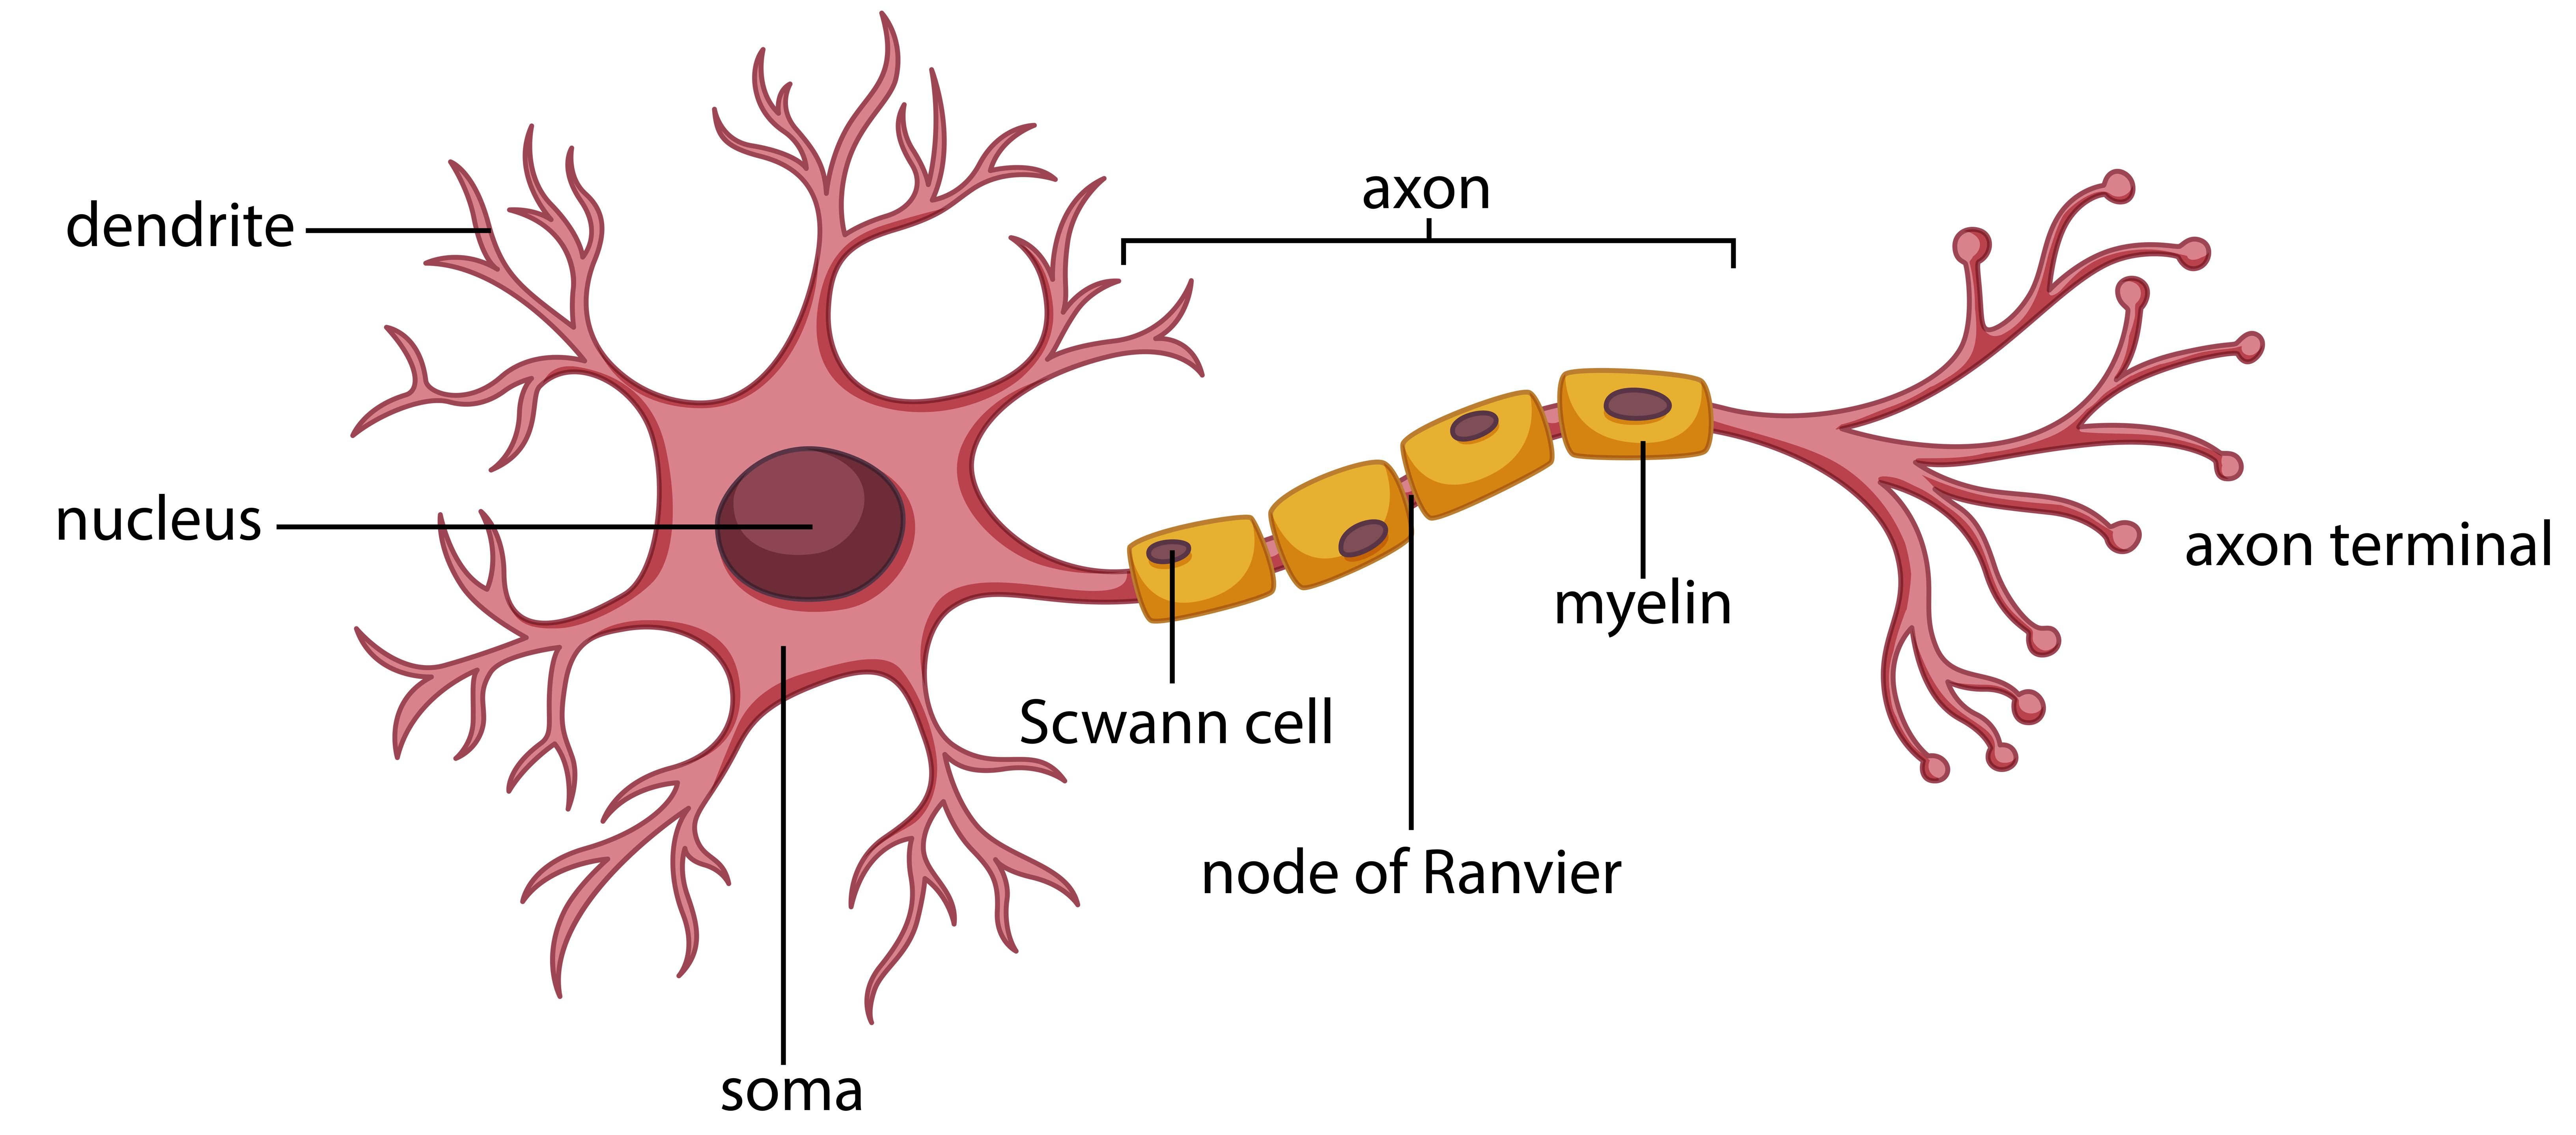
\includegraphics[width=0.8\textwidth]{./figure/neuron_anat.jpg}
        \caption{Neuron anatomy with different componentso}
    \end{figure}
\end{frame}
\begin{frame}{Introduction}
    \begin{itemize}
        \item State of the neuron is defined by the potential of its membrane.
        \item The action potential (the electrical spike released by the neuron) is the result of the depolarization of the membrane.
        \item The action potential is characteristic of the neuron and is used to communicate with other neurons.
        \item The goal of a spikesorter is to identify the action potential of each neuron in the recorded data (record with electrodes).
    \end{itemize}
\end{frame}
\begin{frame}{Introduction}
    \begin{figure}[H]
        \begin{center}
            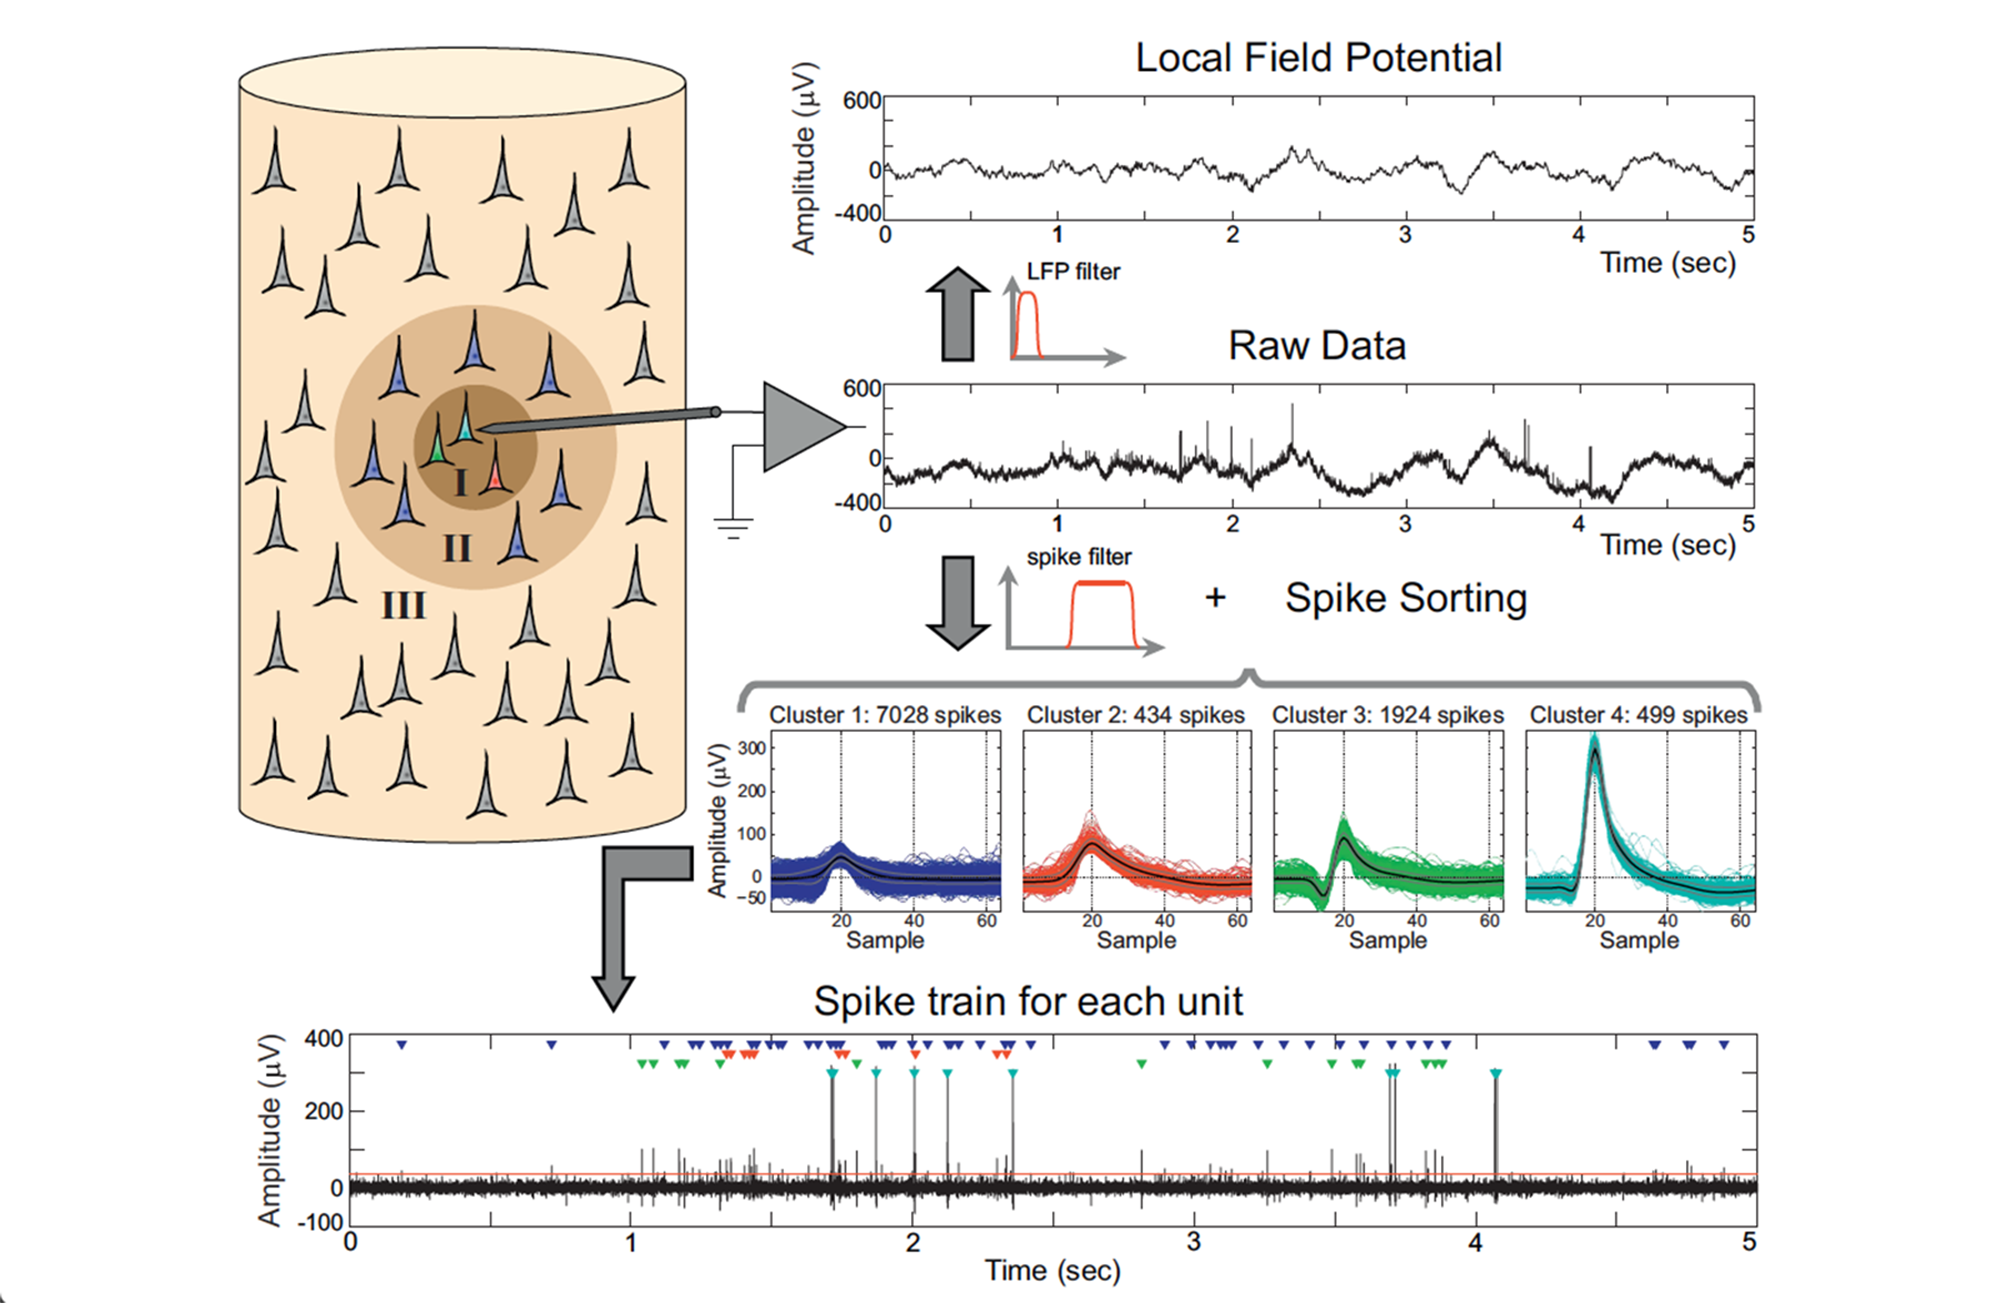
\includegraphics[width=0.8\linewidth]{./figure/spike.png}
        \end{center}
        \caption{\scriptsize{Spike sorting analysis Principles of neurons. The local field potential contains multiple neuron signals, the goal of the spilesorting algorithm is to
                isolate each signal and to attribute each spikes in the local field to a specific neuron. There is many methods to do so. Lussac goal is to deal with multiple of these algorithms to extract the best from each.}}
        \label{fig:}
    \end{figure}
\end{frame}
\begin{frame}{Introduction}
    \begin{itemize}
        \item The spikesorting is a complex problem, and there is no unique solution.
        \item The goal of the Lussac project is to develop a new spikesorting algorithm that will be able to deal with multiple spikesorting algorithms.
        \item The goal of this project is optimize the Lussac choice between the different spikesorting algorithms.
    \end{itemize}
\end{frame}
\section{The Lussac sorting : clustering group of neurons}
\begin{frame}{clustering group of neurons}
    \begin{itemize}
        \item  Identify which neurons are identical between each analysis
        \item process each cluster of the same \emph{real neuron}
        \item deal with relations between nodes of the Lussac graph
        \item each neuron of each analysis is a node of the graph
        \item each edge of the graph stands for relations between two neurons over different metrics
    \end{itemize}
\end{frame}
\subsection{Clustering on low dimensinal space}
\subsubsection{Graph Space}
\begin{frame}{Graph Space}
    \begin{itemize}
        \item The graph space is a i dimensional space with i the number of metrics to compare neurons.
        \item Metrics helps us to determined if a relation between two neurons is good or not
        \item If the relation is good, neurons are part of the same cluster
    \end{itemize}
\end{frame}
\subsubsection{Clustering Metrics}
\begin{frame}{Clustering Metrics}
    \begin{itemize}
        \item Similarity metrics :     $$\text{sim}(n_i, n_j) = \frac{N_{ij}}{\min (N_i, N_j)}$$
              measures the spiking activity similarity between two neurons.
        \item Correlogram difference : Compares the correlogram of two neurons.
              $$\text{corr}_i = \frac{|\Gamma_i - \Gamma_{ij}|}{w_j - w_i}$$
        \item Template difference : Compares the waveform of the two neurons. It is just a euclidean distance, between the two curve.
    \end{itemize}
\end{frame}
\begin{frame}{Clustering Metrics}
    \begin{itemize}
        \item Asymmetric metrics : $$\text{asym}(n_i, n_j) = \frac{N_{ij}}{N_i}$$
              measures the spiking activity similarity between two neurons.
        \item Cross-contamination : Number of violation of the refractory period (rest time of the neuron), corrected by the censure time of the spike-sorter (cannot detect spike that are too close).
    \end{itemize}
\end{frame}
\subsubsection{Unsupervised Clustering}
\begin{frame}{Unsupervised Clustering}
    \begin{itemize}
        \item The goal of the unsupervised clustering is to find the best cluster of neurons.
        \item Unsupervised clustering is a method of clustering that does not require the user to specify clusters for training of the model.
        \item KMEANS is a popular unsupervised clustering algorithm
    \end{itemize}
\end{frame}
\begin{frame}{Unsupervised Clustering}
    \begin{figure}[H]
        \centering
        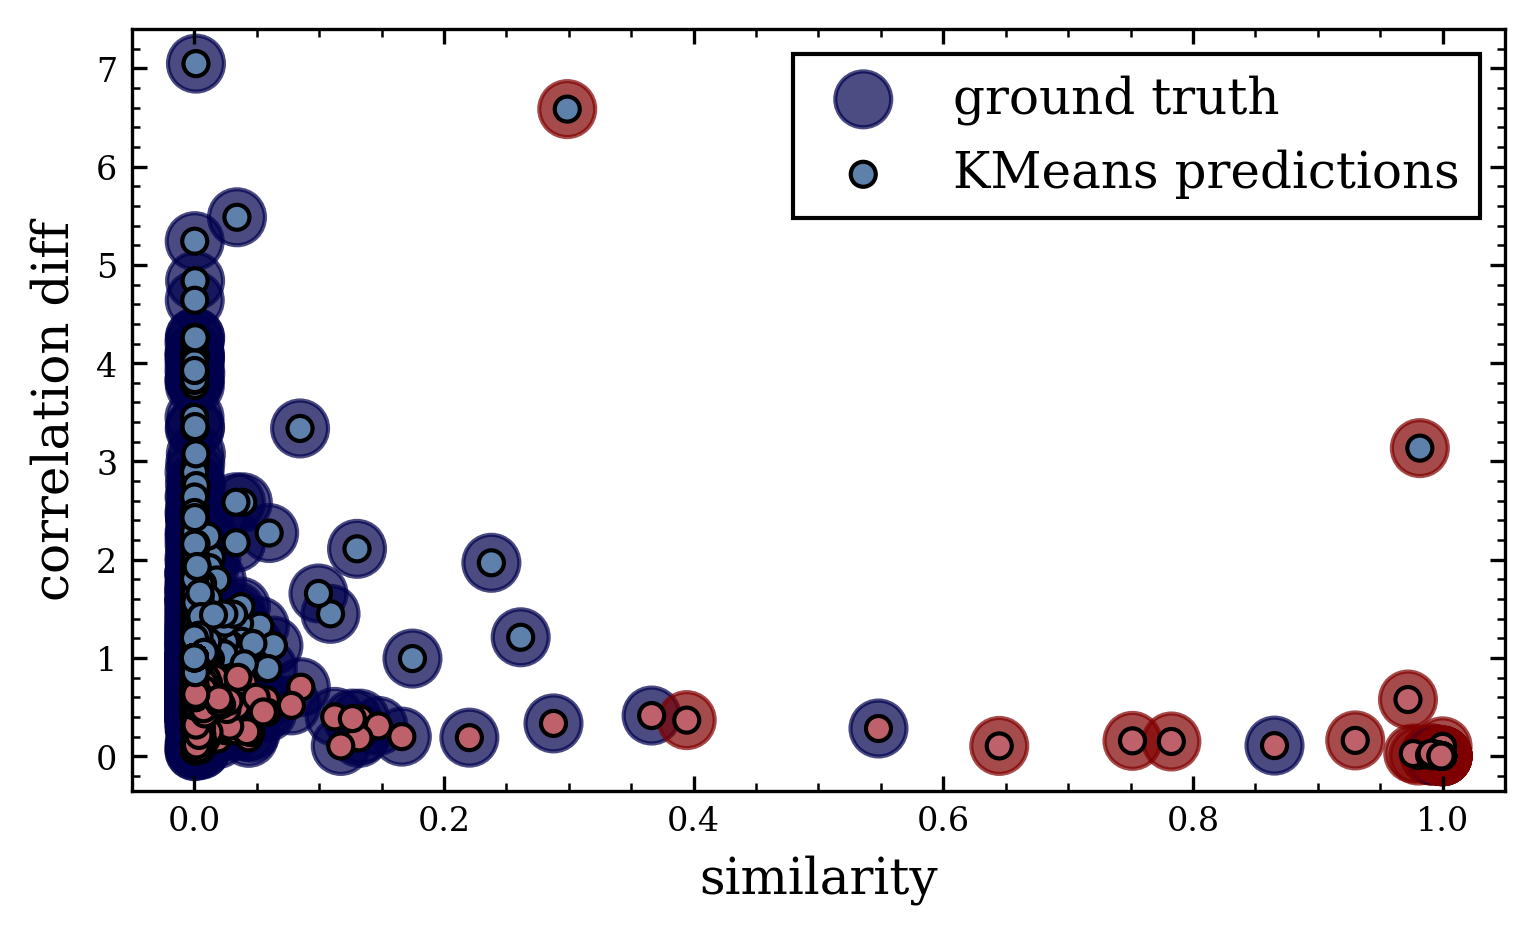
\includegraphics[width=.7\linewidth]{./figure/param_space_km.png}
        \caption{\scriptsize{Big circles are the ground truth label, red one are known good relations between neurons. The results of the unsupervised clustering is
                represented by the little blue and red circle, the red one are the good relations, and the blue one are the bad ones. The unsupervised clustering is not able to separate the data in a good way.)}}
    \end{figure}
\end{frame}
\subsubsection{Supervised Clustering}
\begin{frame}{Supervised Clustering}
    \begin{itemize}
        \item Here the idea is to first use a classification methods to first determine if the edge is good or not.
        \item Then we can use the result of the classification to determine the cluster of the neurons.
        \item The classification methods are trained on a known set of good and bad relations.
        \item Use of SVM classifier (support vector machine)
    \end{itemize}
\end{frame}
\begin{frame}{Supervised Clustering}
    \begin{minipage}{.48\textwidth}
        \begin{figure}[H]
            \centering
            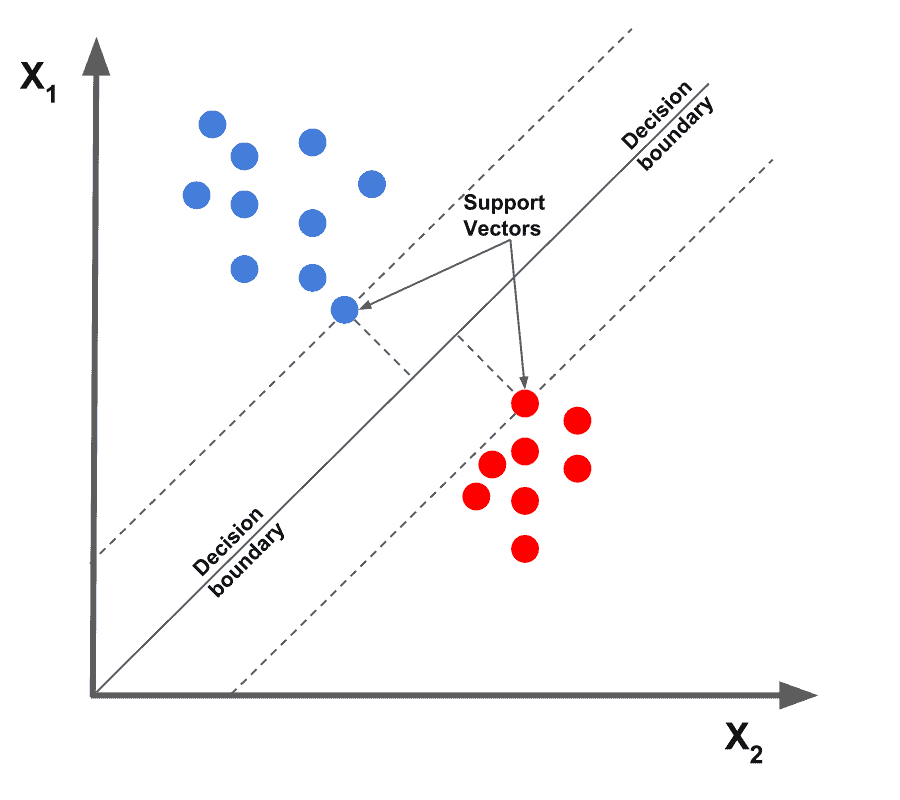
\includegraphics[width=1\linewidth]{./figure/support-vectors-and-maximum-margin.png}
        \end{figure}
    \end{minipage}
    \begin{minipage}{.48\textwidth}
        \begin{itemize}
            \item The SVM classifier find the best hyperplane to separate the data.
            \item Kernel trick is used to separate the data in a higher dimensional space. (non-linear speration)
                  $$K(x_i, x_j) = \exp(-\gamma ||x_i - x_j||^2)$$

        \end{itemize}
    \end{minipage}
\end{frame}
\begin{frame}{application}
    \begin{figure}[H]
        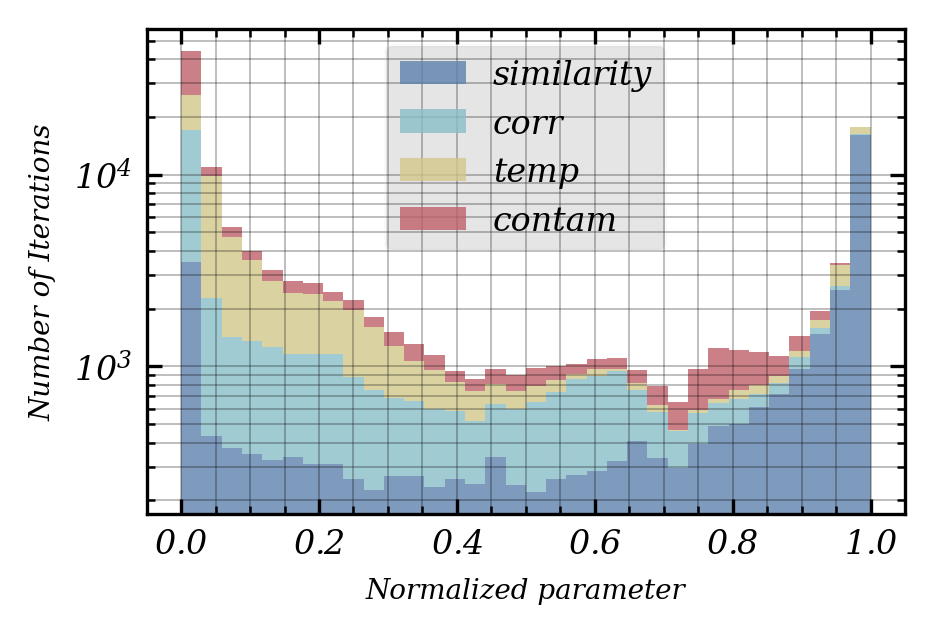
\includegraphics[width = .6\linewidth]{./figure/param_distrib.png}
    \end{figure}
    \begin{itemize}
        \item features distribution study
        \item appears that template difference and contamination are quite redundant in their distribution
    \end{itemize}
\end{frame}
\begin{frame}{application}
    \begin{figure}[H]
        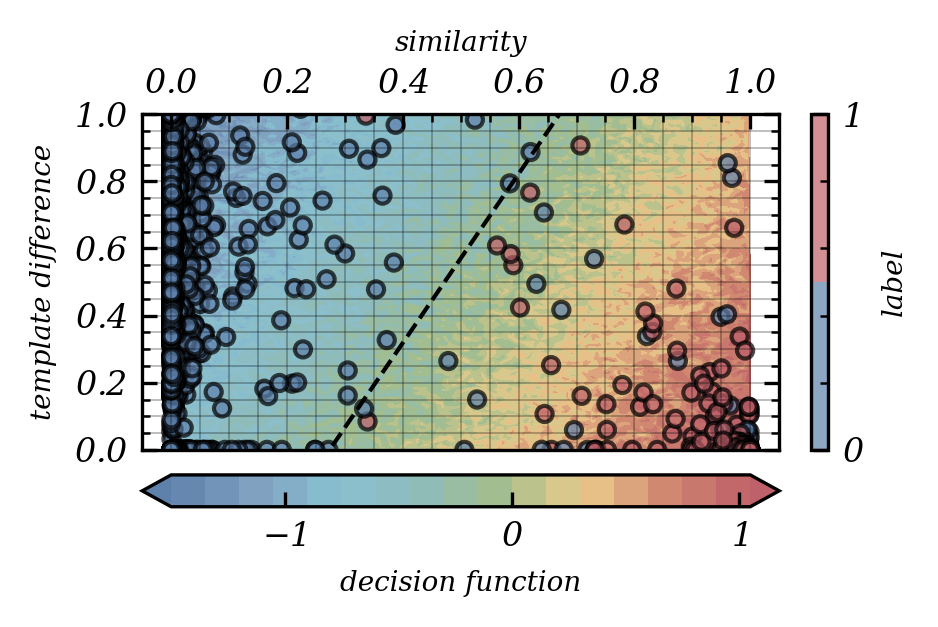
\includegraphics[width = .5\linewidth]{./figure/decision_function.png}
        \caption{\scriptsize{Decision Function for the given SVM, the correlation dependence is omitted due to its weak impact on the decision boundaries}}
    \end{figure}
    \begin{itemize}
        \item able to separate the data in a good way
        \item score of 0.9997 on the test set : really bad neurons are numerous and easy to separate from the good ones.
        \item Introduce new metrics to have better insights of the classification
    \end{itemize}
\end{frame}

\begin{frame}{application}
    \begin{figure}[H]
        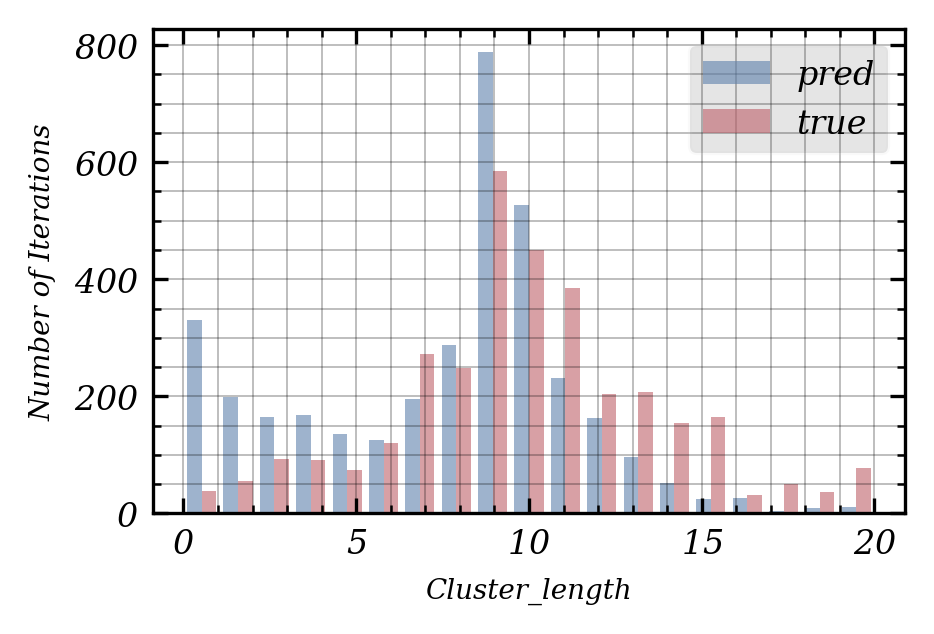
\includegraphics[width = .6\linewidth]{./figure/cluster_length.png}
        \caption{\scriptsize{Here we can see the length histogram of the clusters, the length of the clusters is the number of neurons inside this latter. In blue the predicted cluster length and in red the true one.}}
    \end{figure}
    \begin{itemize}
        \item predicted clusters have the same distribution as the true one
        \item smaller size of the clusters : relevant for eliminate bad units
    \end{itemize}
\end{frame}
\begin{frame}{Clustering Efficiency}

    \begin{itemize}
        \item quantify clustering quality
        \item use the following formula :     $$ \text{score}(Y^{\text{pred}}, Y^{\text{true}}) = \sum_{k=0}^N \frac{ \# (G_k^{\text{pred}} \cap  G_k^{\text{true}})}{\max (\# G_k^{\text{pred}}, \# G_k^{\text{true}})}$$
        \item from this we get a score of 0.94 for the SVM classifier
    \end{itemize}
\end{frame}
\subsection{Clustering on high dimensional space}
\begin{frame}{Clustering on high dimensional space}
    \begin{itemize}
        \item expand dimsensions to separate the data in a better way
        \item Next we will just keep the similarity, template difference, correlogram difference metrics to simplify the problem. The features space is then of dimension 3.
        \item gives the following representation of the data :
              $$
                  \underbrace{
                      \begin{pmatrix}
                          |1,0,0| & \dots   & \dots   \\
                          \dots   & |1,0,0| & \dots   \\
                          \dots   & \dots   & |1,0,0| \\
                      \end{pmatrix}}_{3N}
              $$
        \item In this representation we do not consider the link validity but how the neuron are connected together.
    \end{itemize}
\end{frame}
\subsubsection{Various Unsupervised Algorithm}
\begin{frame}{Various Unsupervised Algorithm}
    \begin{itemize}
        \item Affinity Propagation
        \item HDBSCAN
        \item both methods lead to poor score compared to the SVM classifier (respectively 0.687 and 0.781)
        \item eliminate neurons for mid-size cluster which is not relevant
    \end{itemize}
\end{frame}
\section{Nodes Clustering}
\subsection{Nodes space}
\begin{frame}{Nodes Clustering}
    \begin{itemize}
        \item the nodes clustering is the next step of the Lussac algorithm
        \item After creating clusters based on neurons relations
        \item We want to isolate the best neurons of each cluster, to have the best representation of the real neurons.
    \end{itemize}
\end{frame}
\subsection{Different methods}
\begin{frame}{metrics Overview}
    \begin{itemize}
        \item \textbf{rb contamination} : The contamination gives a corrected number of violations metrics, indeed it's calculated using a censure time. Indeed, spike sorters are not able to detect spikes that are too close to each other. A way of correct the rate of number of violation is to not consider a specific time window around each spike. This time window is called the censure time.
        \item \textbf{SNR} : The SNR is the ratio between the mean of the spike amplitude and the standard deviation of the noise. The SNR is a measure of the quality of the spike detection. A high SNR means that the spike detection is good.

    \end{itemize}
\end{frame}

\begin{frame}{metrics Overview}
    \begin{itemize}

        \item \textbf{presence ratio} : The presence ratio is the ratio between the number of spikes detected and the number of spikes expected. A high presence ratio means that the spike detection is good.
        \item \textbf{firing rate} : The firing rate is the number of spikes detected divided by the duration of the recording. A high firing rate means that the spike detection is good.
        \item \textbf{synchrony} : The synchrony is the ratio between the number of coinciding spikes and the number of spikes detected. A high synchrony means that the spike detection is good.

    \end{itemize}
\end{frame}

\begin{frame}{metrics Overview}
    \begin{itemize}

        \item \textbf{sd ratio} : The sd ratio is the ratio between the standard deviation of the spike amplitude and the standard deviation of the noise. A high sd ratio means that the spike detection is good.
        \item  \textbf{quality score metrics} :  The quality metrics is score taking into account the contamination and the number of spikes (firing rate). It is defined as following :
              $$S = N(1 - (k+1)C)$$ witth $N$ the number of spikes, $C$ the contamination and $k$ a constant. Generally we take $k = 1$ for minimizing the accuracy, but one could argue that it's not the best choice, indeed a false positive has a stronger impact on the spike sorting quality,
              so we could take $k = 2.5$ to accentuate the dependence of false positive on the score. Indeed, the former formula leads to : $$S = N - FN - k FP$$.
    \end{itemize}
\end{frame}
\begin{frame}
    \begin{minipage}{.6\textwidth}
        \begin{figure}[H]
            \centering
            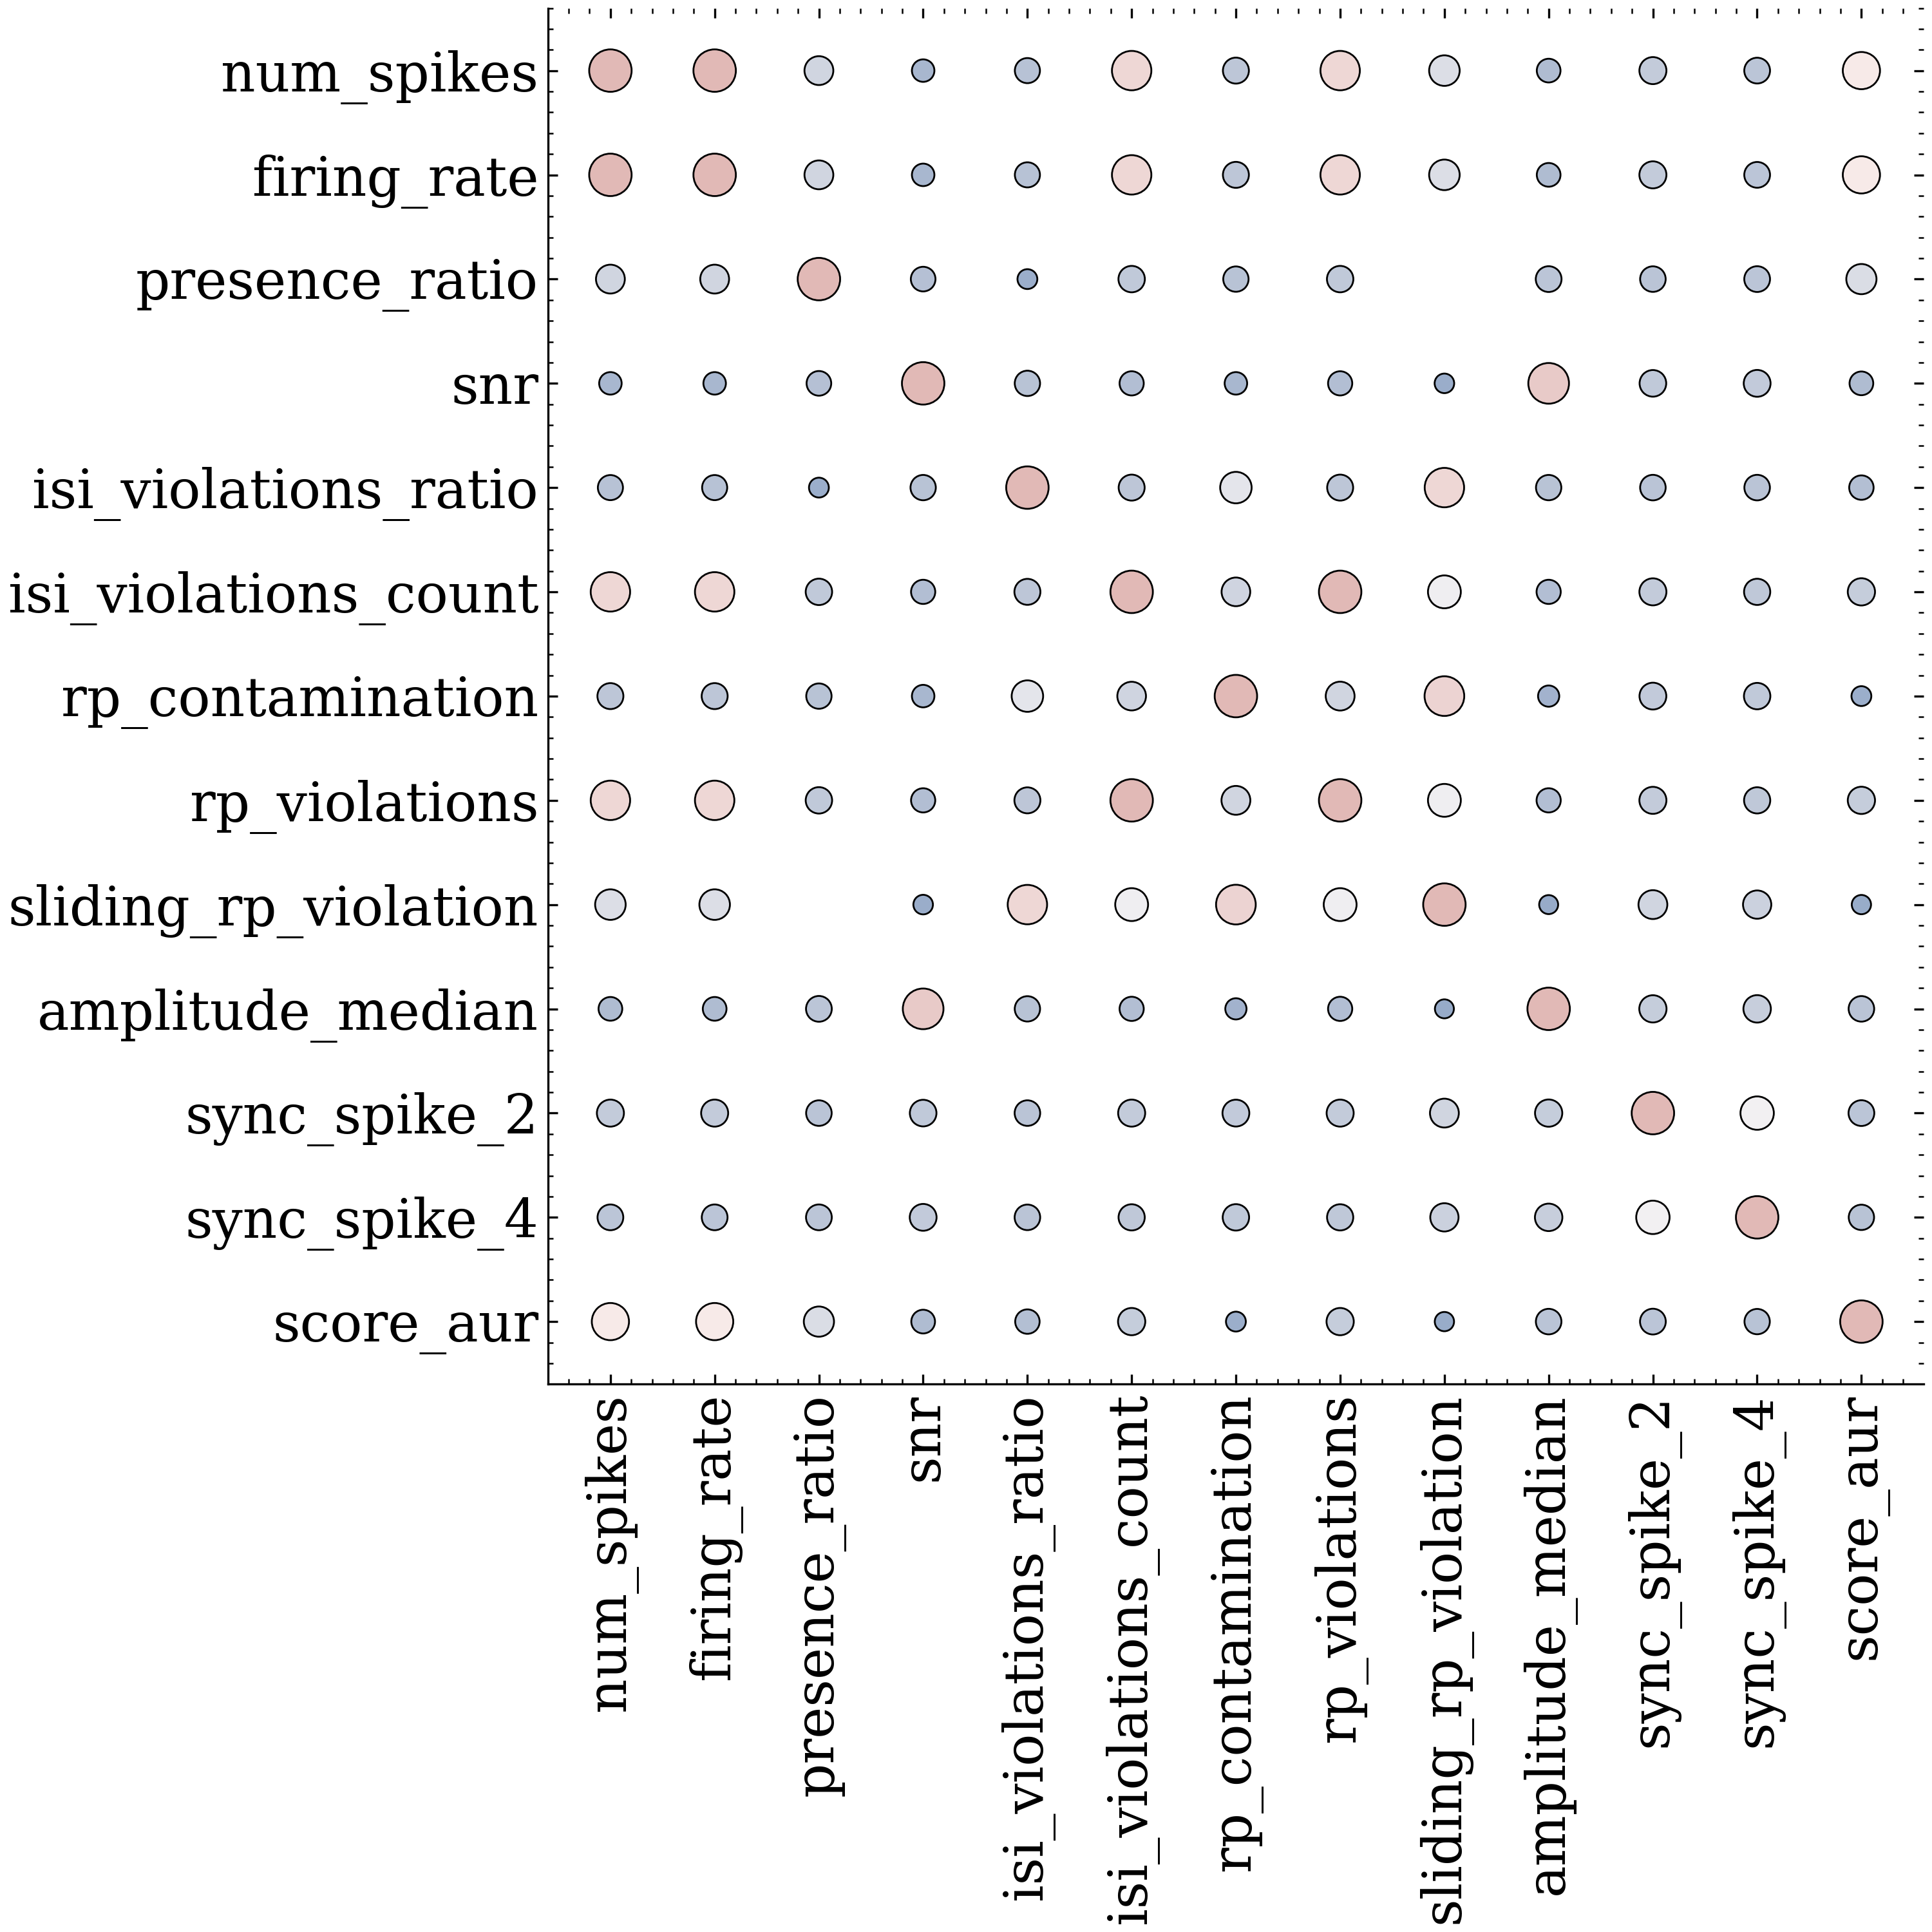
\includegraphics[width=1\linewidth]{./figure/correlation.png}
            \caption{\scriptsize{Correlation matrix of the different metrics}}
            \label{}
        \end{figure}
    \end{minipage}
    \begin{minipage}{.38\textwidth}
        \begin{itemize}
            \item goal is to keep the most relevant uncorrelated metrics
            \item sd ratio and SNR are highly correlated
            \item presence ratio and firing rate are highly correlated
        \end{itemize}
    \end{minipage}
\end{frame}
\subsection{Clustering on every nodes}
\begin{frame}{Clustering on every nodes}
    \begin{itemize}
        \item Dropping the cluster dependence allows us to use all the nodes for the global clustering
        \item Some metrics are cluster dependent, so we have to drop them
        \item We used the following : SNR, contamination, presence ratio
    \end{itemize}
\end{frame}

\begin{frame}{Weighting Function}
    \begin{itemize}
        \item To avoid a strong impact of near best neurons on the clustering, we use a weighting function
              $$f(x) = \left[\tanh \left( \frac{x - \text{max}_c /W_C}{\sigma} \right) + \frac{1}{2} \right]^2$$
              x is the known accuracy score of the training set
        \item We consider just the best neurons of each cluster and bad neurons.
        \item Best neuron and bad neurons are determined by the accuracy score.
    \end{itemize}
\end{frame}
\begin{frame}{Clustering}
    \begin{minipage}{.48\textwidth}
        \begin{figure}[H]
            \centering
            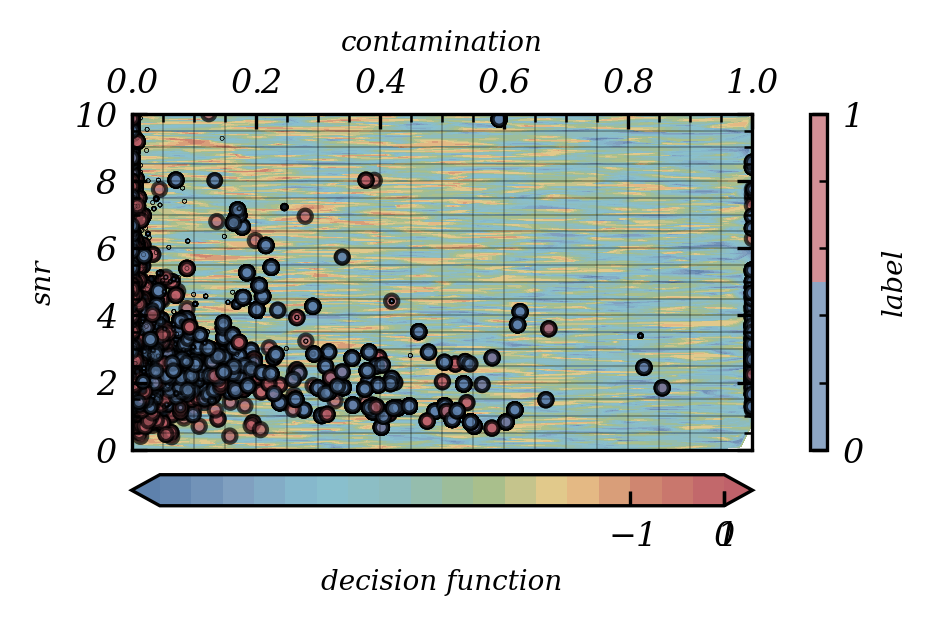
\includegraphics[width=1\linewidth]{./figure/decision_function_working_2.png}
            \caption{\scriptsize{The data is impossible to separate into 2 clusters, the SVM is overfitting the data}}
            \label{}
        \end{figure}
    \end{minipage}
    \begin{minipage}{.48\textwidth}
        \begin{figure}[H]
            \centering
            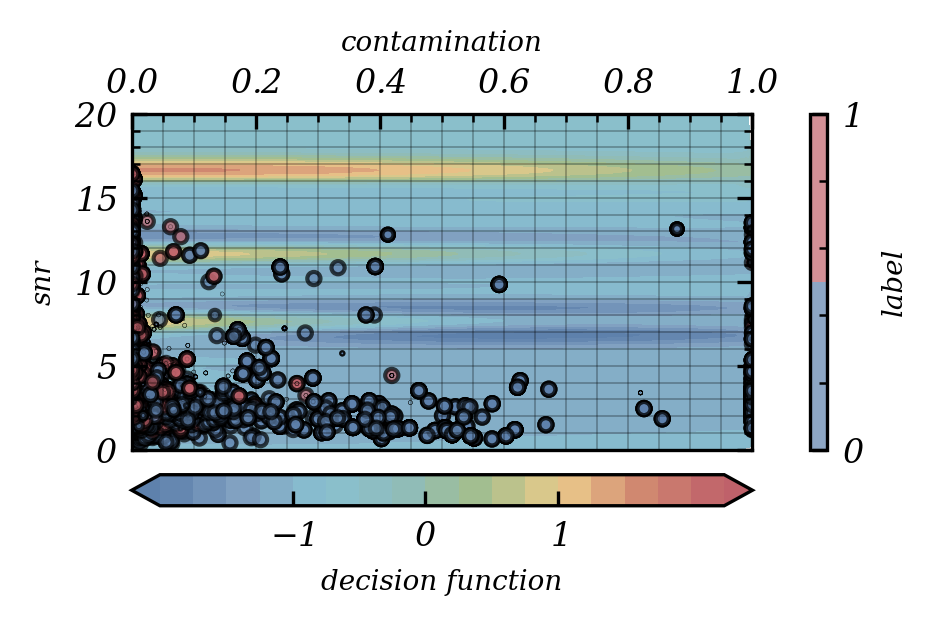
\includegraphics[width=1\linewidth]{./figure/decision_function_working_3.png}
            \caption{\scriptsize{dropping the presence ratio leads to the same results need to introduce relative cluster metrics}}
            \label{}
        \end{figure}
    \end{minipage}
\end{frame}
\subsection{Clustering with relative clusters metrics}
\begin{frame}{Relative Clusters Metrics}
    \begin{itemize}
        \item  one way of solving this is to renormalize the parameter by the mean and the std of the cluster
              $$\frac{p_i - \mu}{\sigma}$$ This way we can compare the different clusters.
              \begin{figure}[H]
                  \centering
                  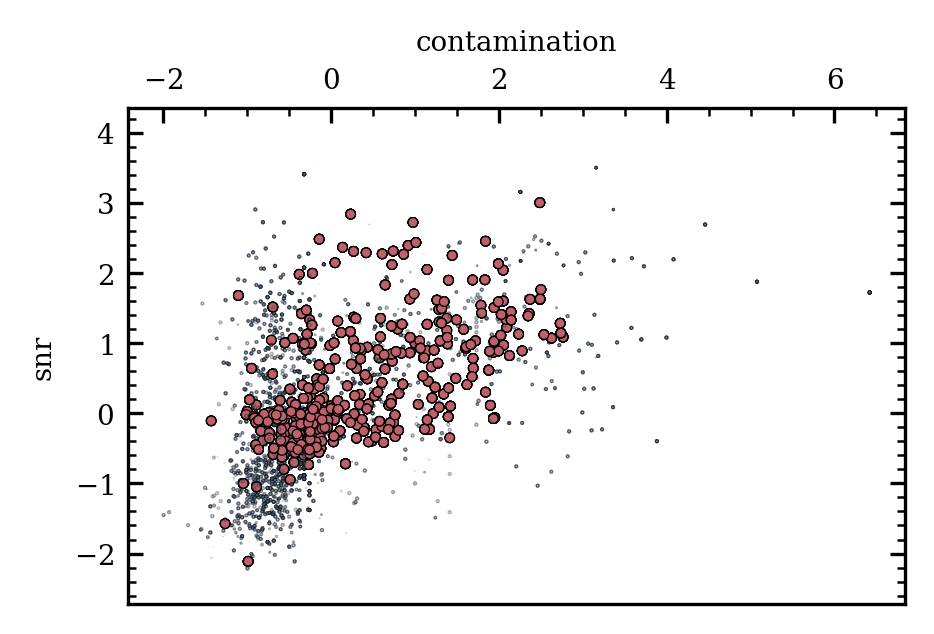
\includegraphics[width=0.6\linewidth]{figure/clusters_weights.png}
                  \caption{\scriptsize{In red the good neurons and in black the bad ones, size of neurons are proportional to their weights. \textbf{Introduce class weights.}}}
                  \label{}

              \end{figure}
    \end{itemize}
\end{frame}
\subsubsection{SVM classifier}
\begin{frame}{SVM classifier}
    \begin{figure}[H]
        \centering
        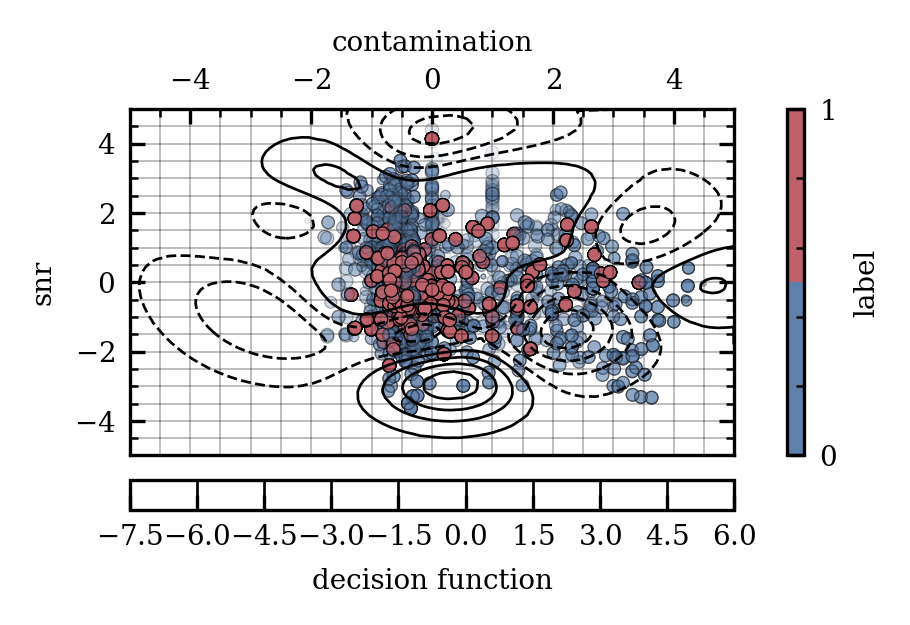
\includegraphics[width=0.6\linewidth]{figure/decision_function_working_6.png}
    \end{figure}
    \begin{itemize}
        \item More homogeneous separation of the data
        \item However the separation is not perfect and one way of improving the separation is to tweak the kernel parameters of the SVM, and the penalty parameter.
    \end{itemize}
\end{frame}

\begin{frame}{SVM classifier}
    \begin{figure}[H]
        \centering
        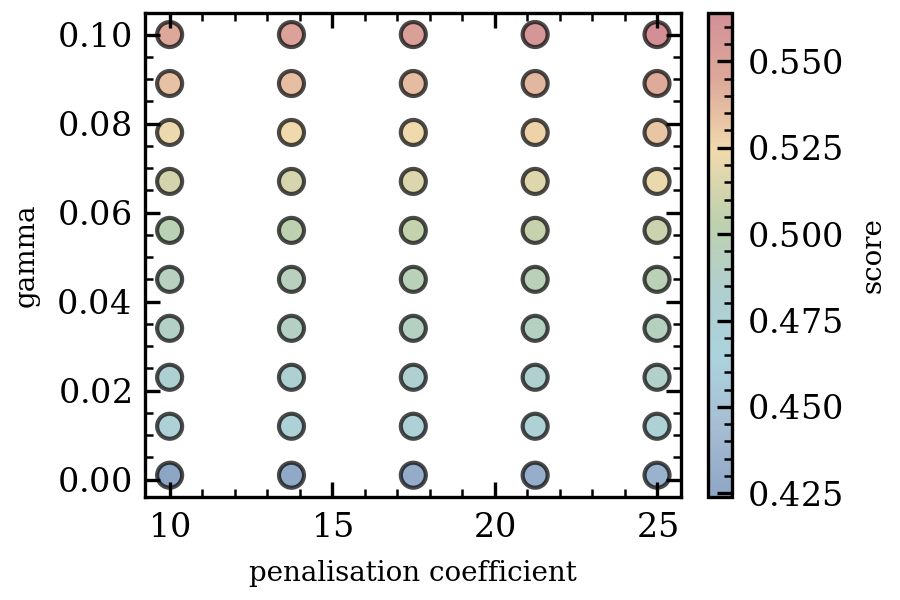
\includegraphics[width=0.6\linewidth]{figure/grid_search.png}
    \end{figure}
    \begin{itemize}
        \item Perform a grid search to find the best parameters for the SVM
        \item this leads to relatively high $\Gamma$ and $C$ parameters
    \end{itemize}
\end{frame}
\begin{frame}{SVM classifier}
    \begin{figure}[H]
        \centering
        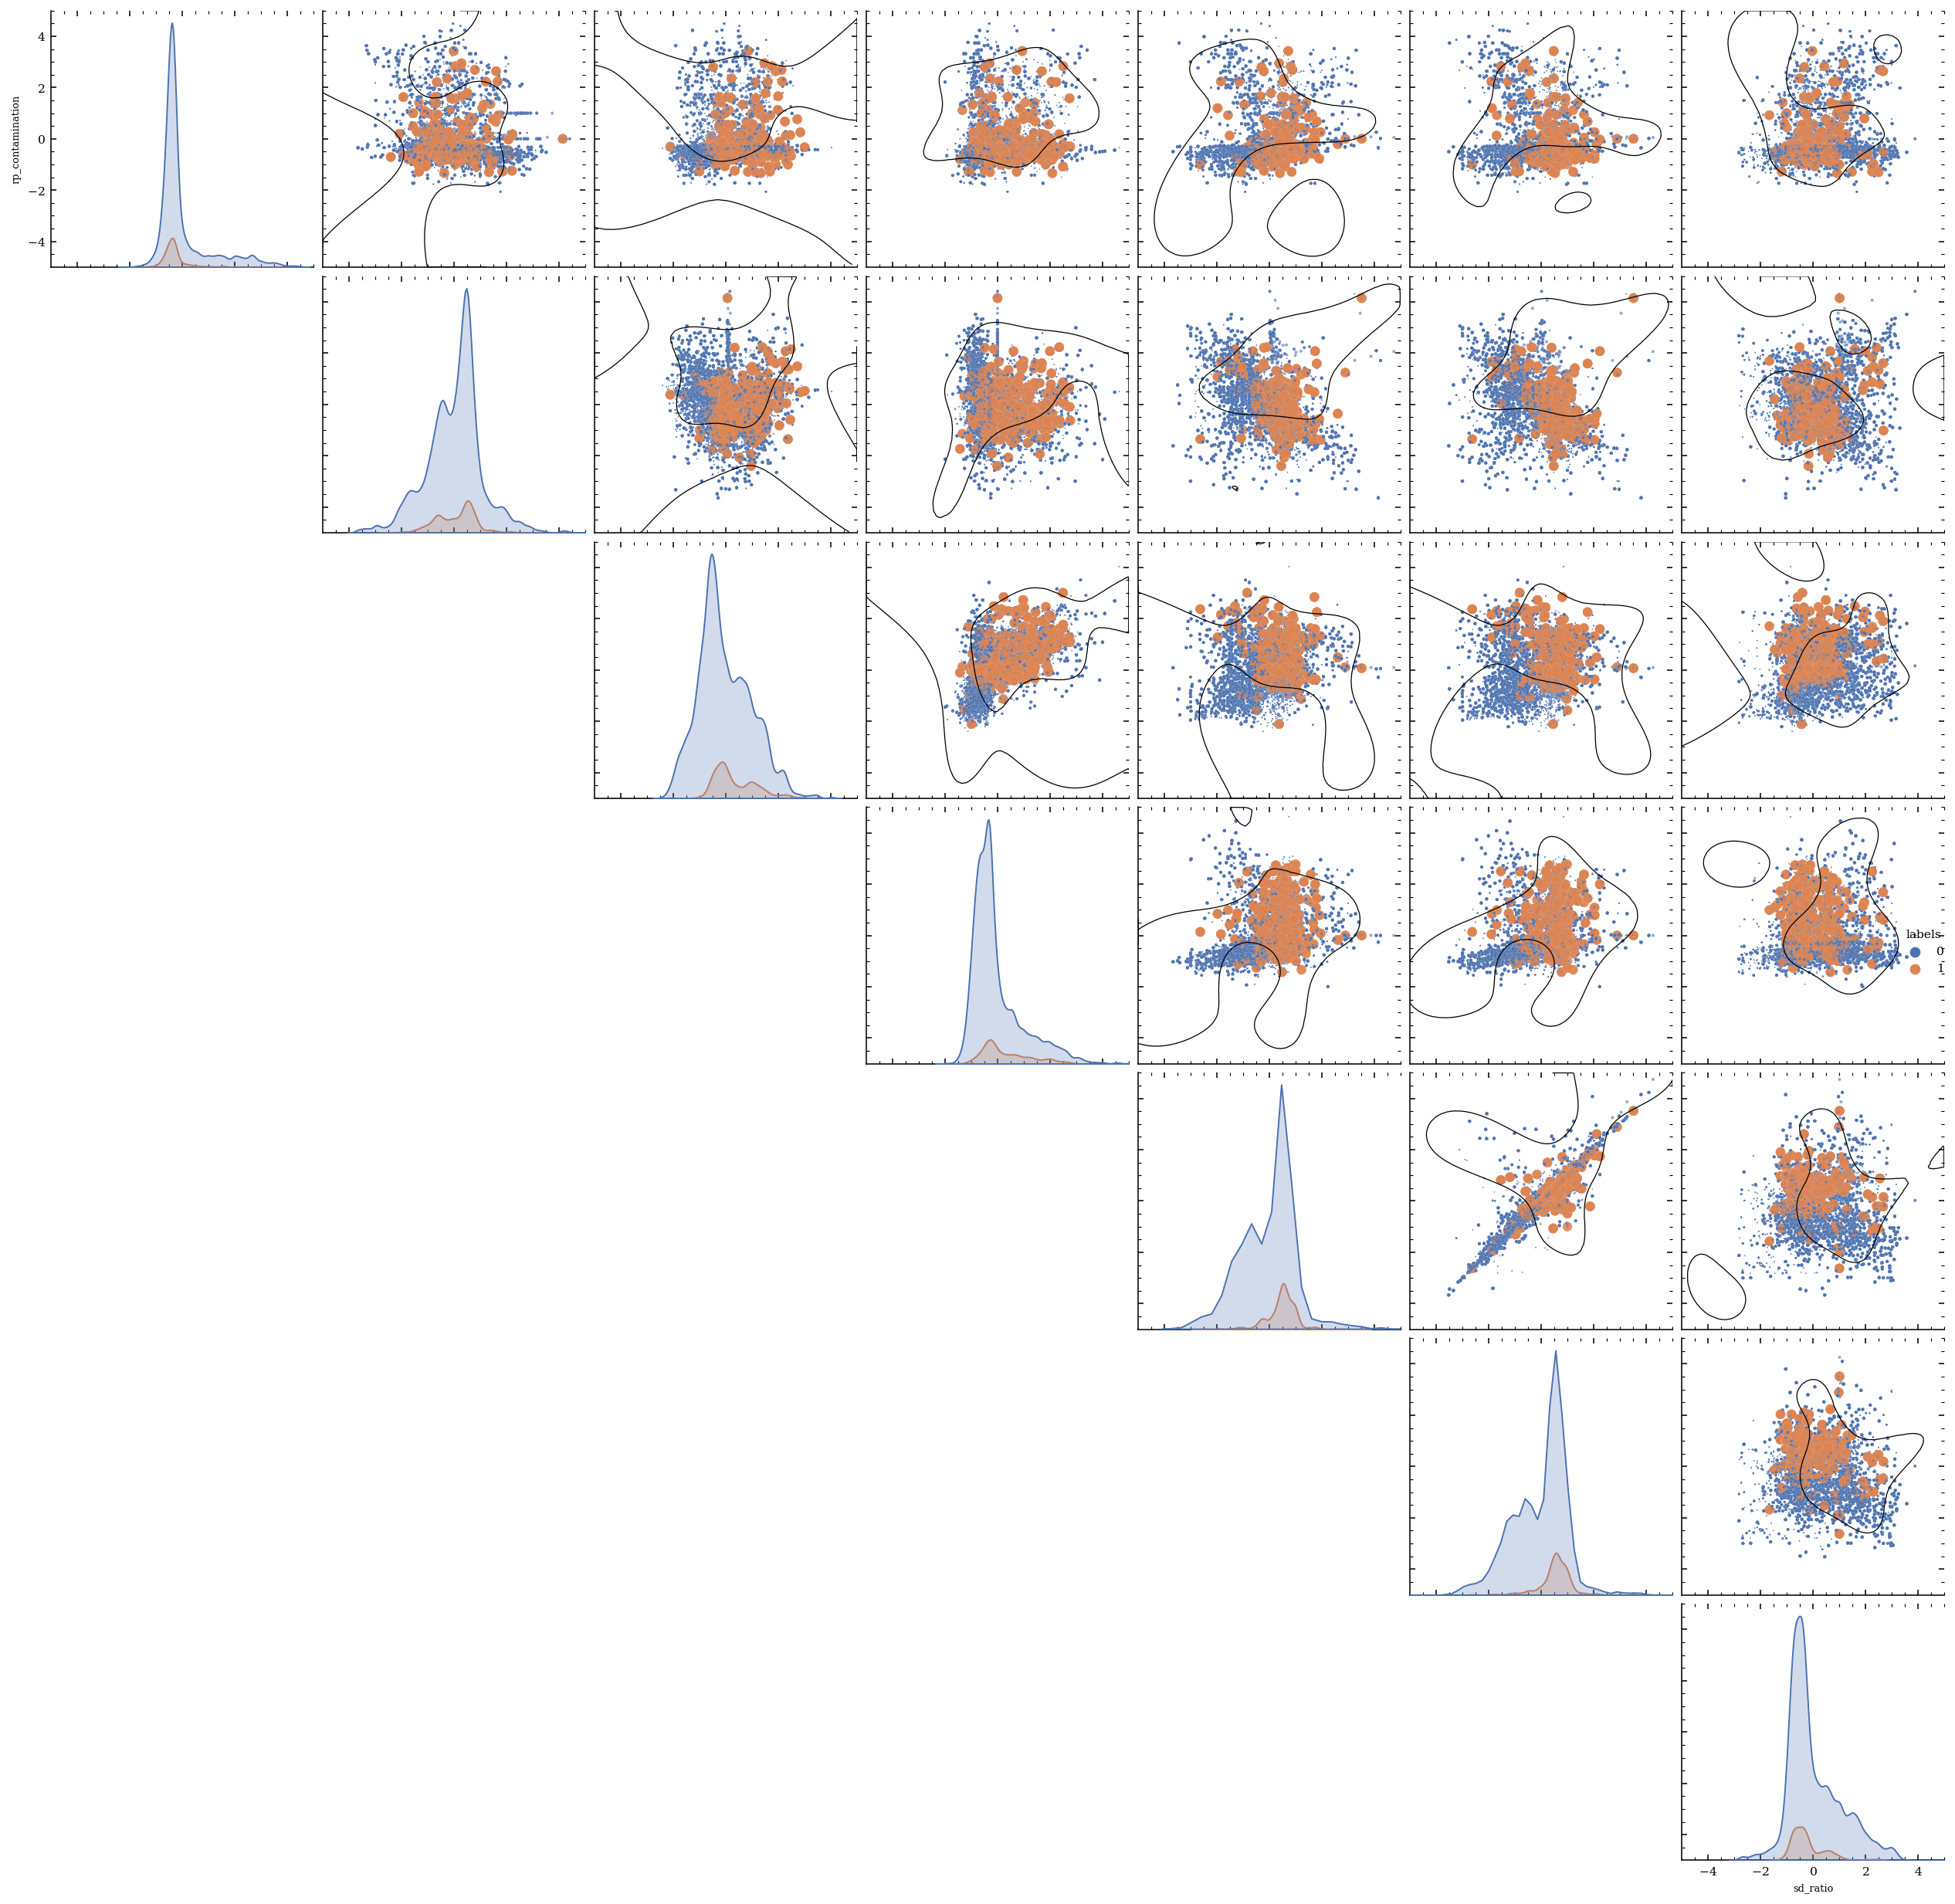
\includegraphics[height=0.6\linewidth]{figure/decision.png}
    \end{figure}
\end{frame}
\begin{frame}{SVM classifier}
    \begin{itemize}
        \item The separation line is too complex
        \item fix the problem by choosing small $\Gamma = 0.03$
              \begin{figure}[H]
                  \centering
                  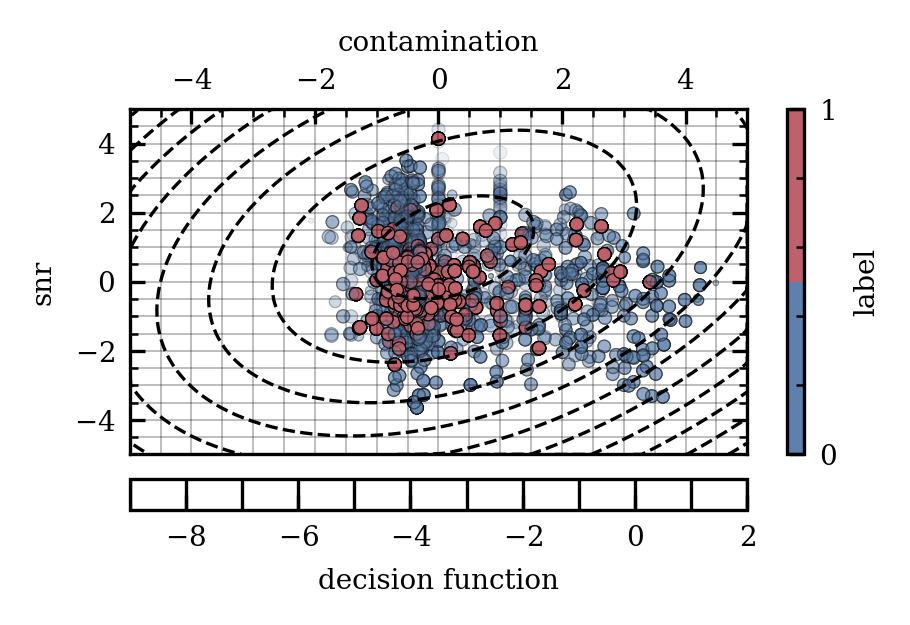
\includegraphics[width=0.7\linewidth]{figure/decision_function_working_5.png}
                  \caption{\scriptsize{Here we choose $\Gamma = 0.03$ and $C = 1$ (i.e. no penalty), the separation line is much more homogeneous.}}
              \end{figure}
    \end{itemize}
\end{frame}
\begin{frame}{SVM Classifier}
    \begin{figure}[H]
        \centering
        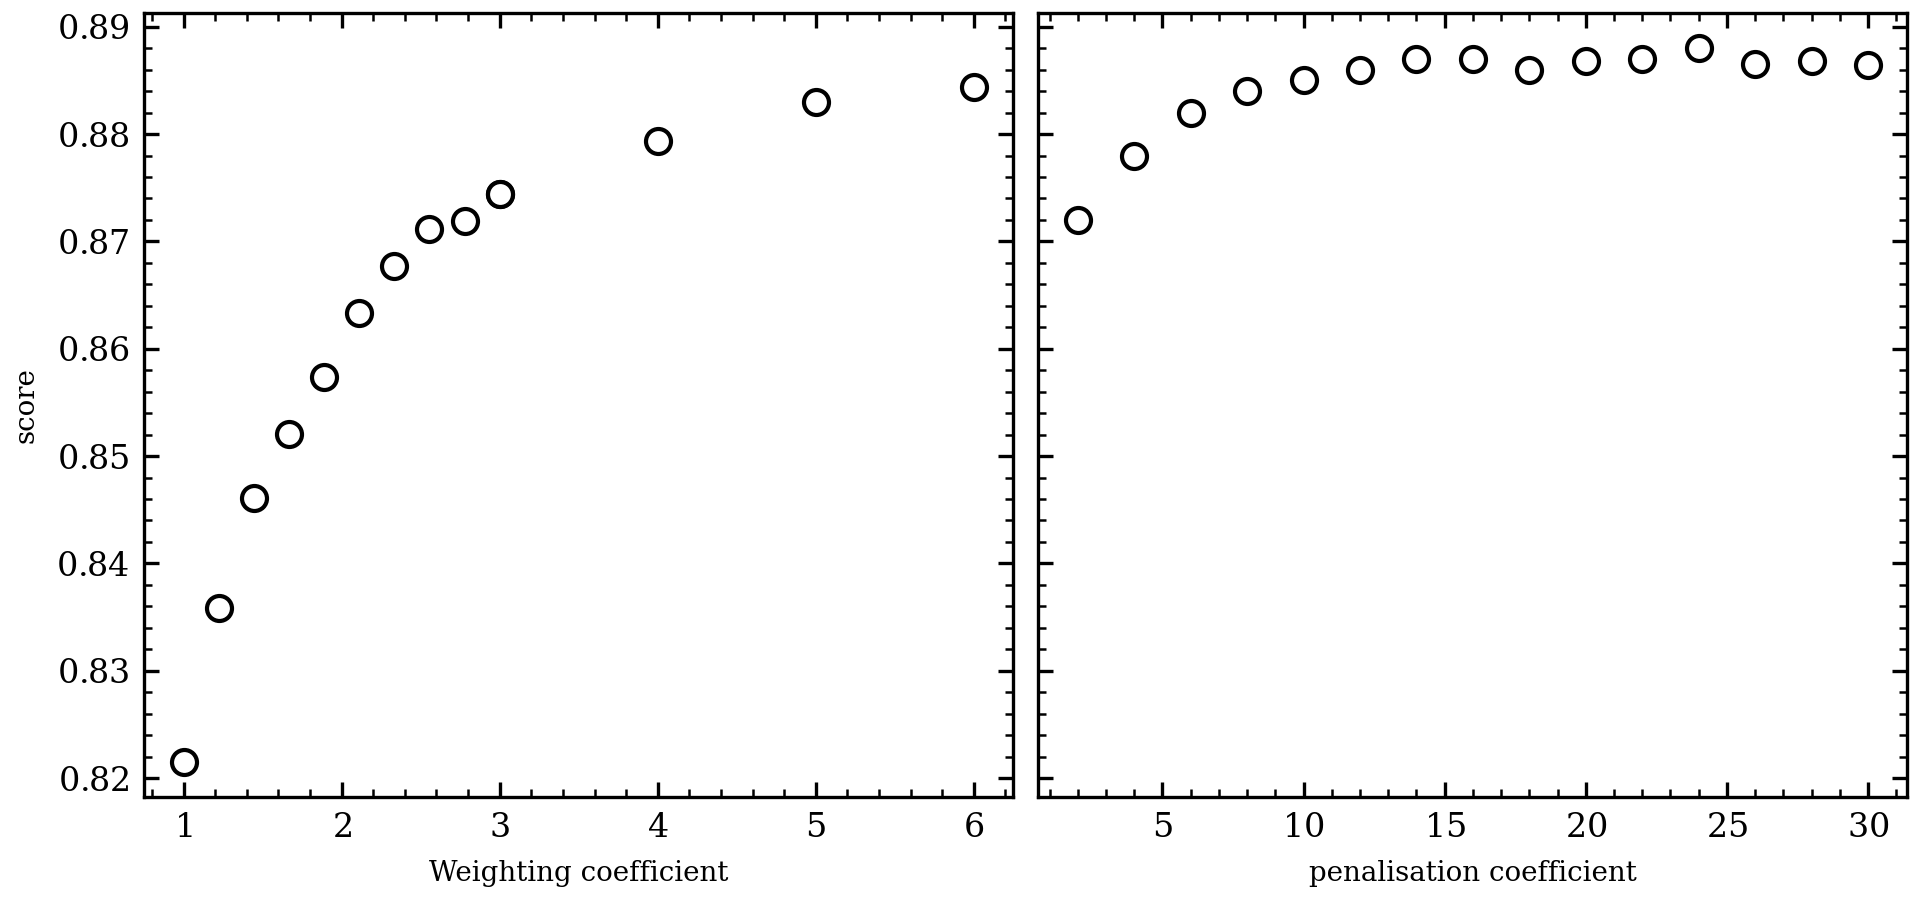
\includegraphics[width=.7\linewidth]{figure/score.png}
    \end{figure}
    \begin{itemize}
        \item optimize with $\Gamma = 0.03$
        \item Must take large penalty and weighting parameter
        \item With $C = W_C = 5$ we got a final score of 0.84
    \end{itemize}
\end{frame}
\subsubsection{Naive Bayes classifier}
\begin{frame}{Naive Bayes classifier}
    \begin{itemize}
        \item Naive Bayes classifier is a simple probabilistic classifier based on applying Bayes' theorem with strong (naive) independence assumptions between the features.
        \item Clustering over \textbf{synchrony} and \textbf{SNR} gives us the following (With the same weighting process as the SVM) :
              \begin{figure}[H]
                  \centering
                  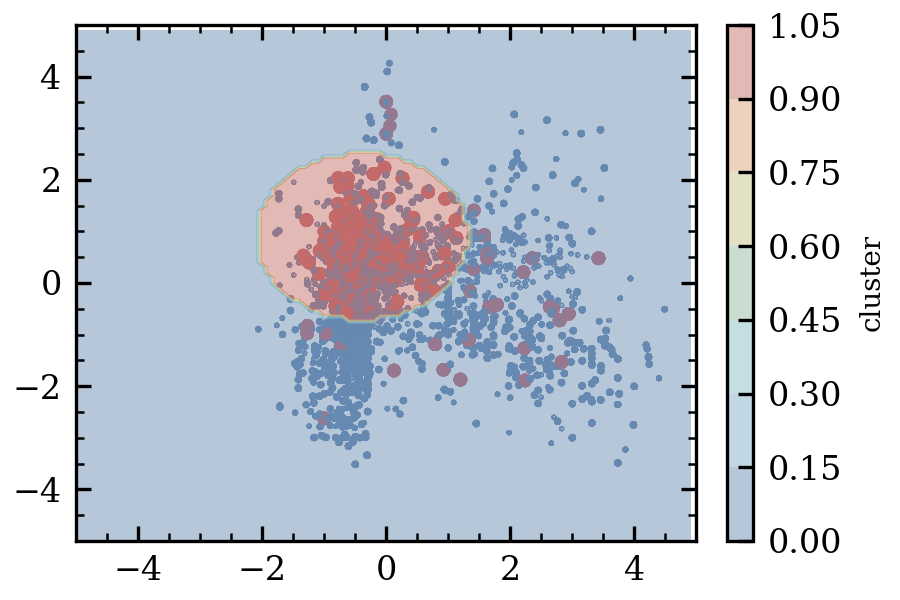
\includegraphics[width=0.6\linewidth]{figure/cluster_GaussianNB.png}
              \end{figure}
    \end{itemize}
\end{frame}
\begin{frame}{Naive Bayes classifier}
    \begin{figure}[H]
        \centering
        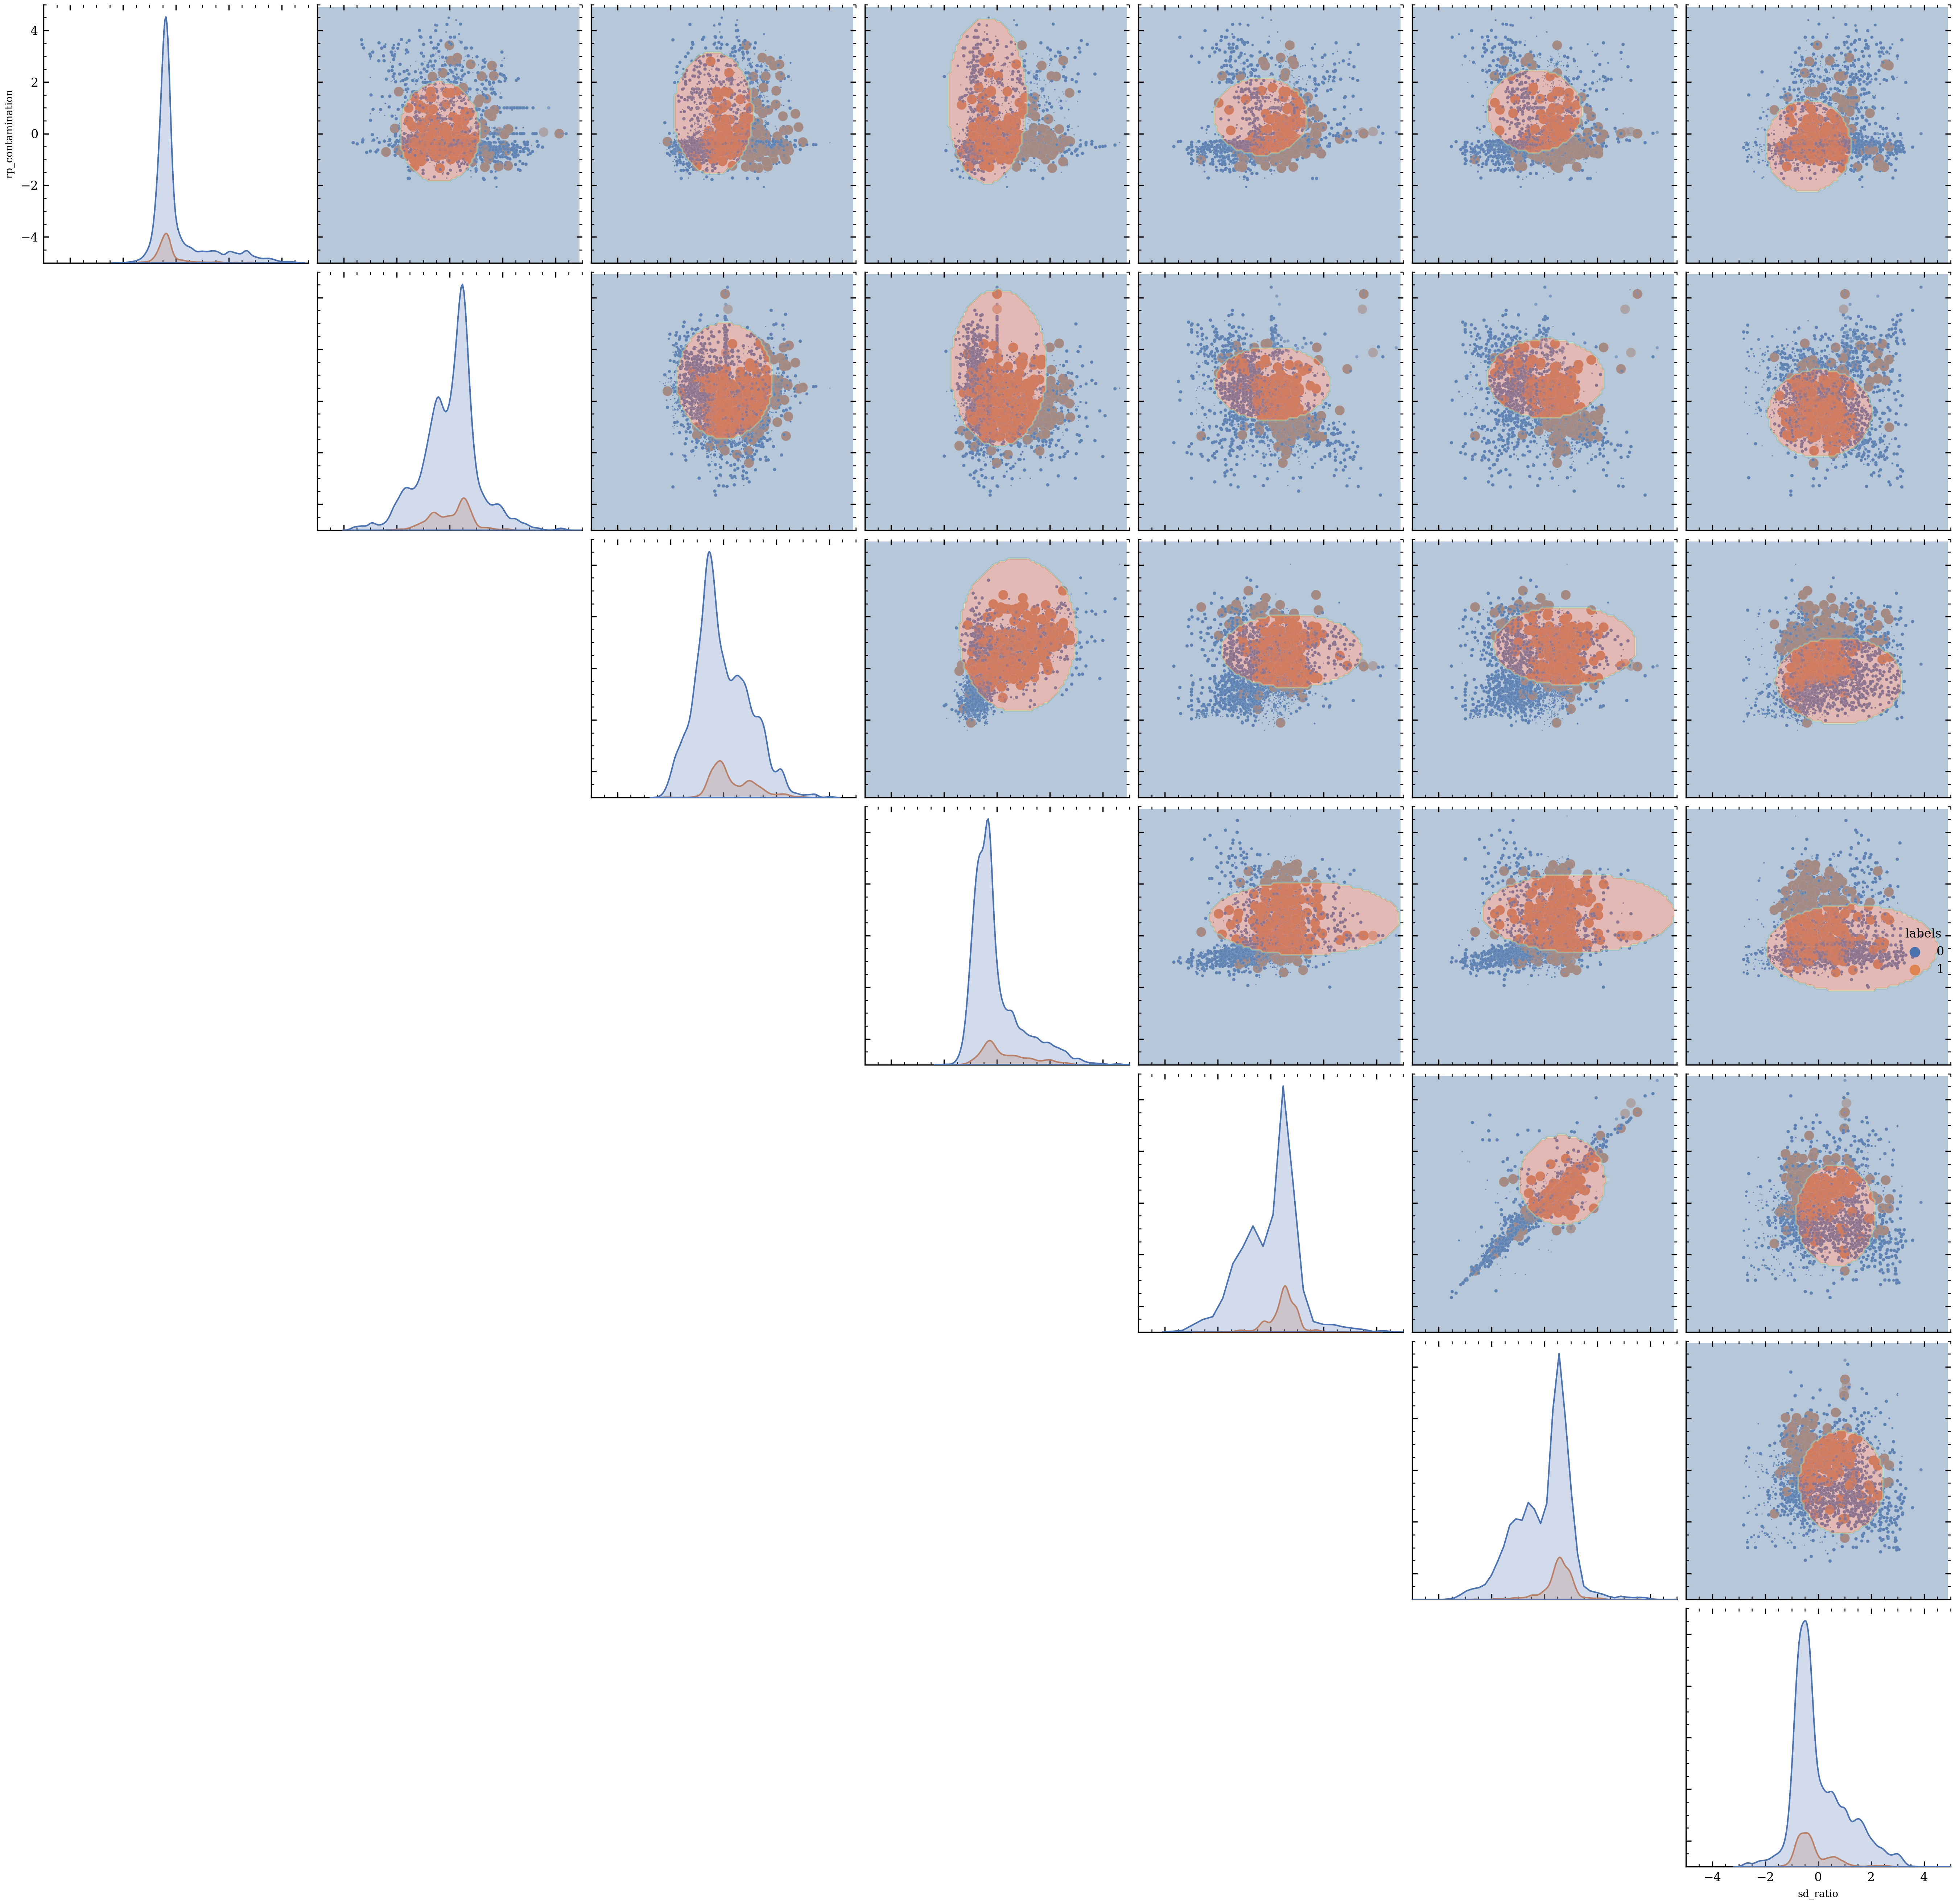
\includegraphics[height=0.6\linewidth]{./figure/Gaussianb_pair.png}
    \end{figure}
\end{frame}
\begin{frame}{Naive Bayes classifier}
    \begin{itemize}
        \item for some diensions the clustering is not perfect.
        \item However, clusters centers are always well separated.
        \item The multidimensional analysis leads to a global score of 0.87, given the weighting metrics.
    \end{itemize}

\end{frame}
\subsubsection{Quadratic Discriminant Analysis}
\begin{frame}{Quadratic Discriminant Analysis}
    \begin{itemize}
        \item Quadratic Discriminant Analysis assumes that the probability density function of the features given the class follows a Gaussian distribution
        \item Clustering over \textbf{synchrony} and \textbf{SNR} gives us the following (With the same weighting process as the SVM) :
              \begin{figure}[H]
                  \centering
                  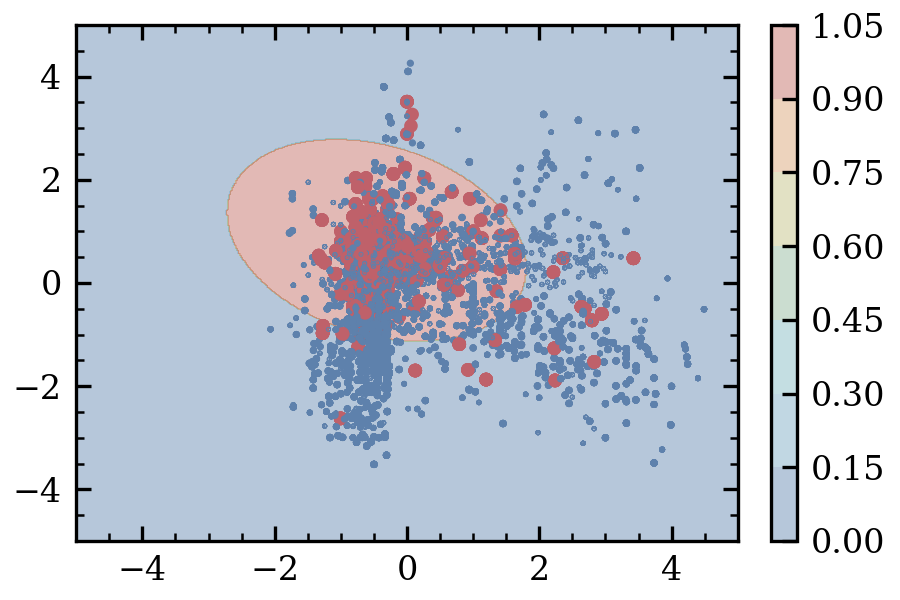
\includegraphics[width=0.6\linewidth]{figure/cluster_qda2.png}
              \end{figure}
    \end{itemize}
\end{frame}
\begin{frame}{Quadratic Discriminant Analysis}
    \begin{figure}[H]
        \centering
        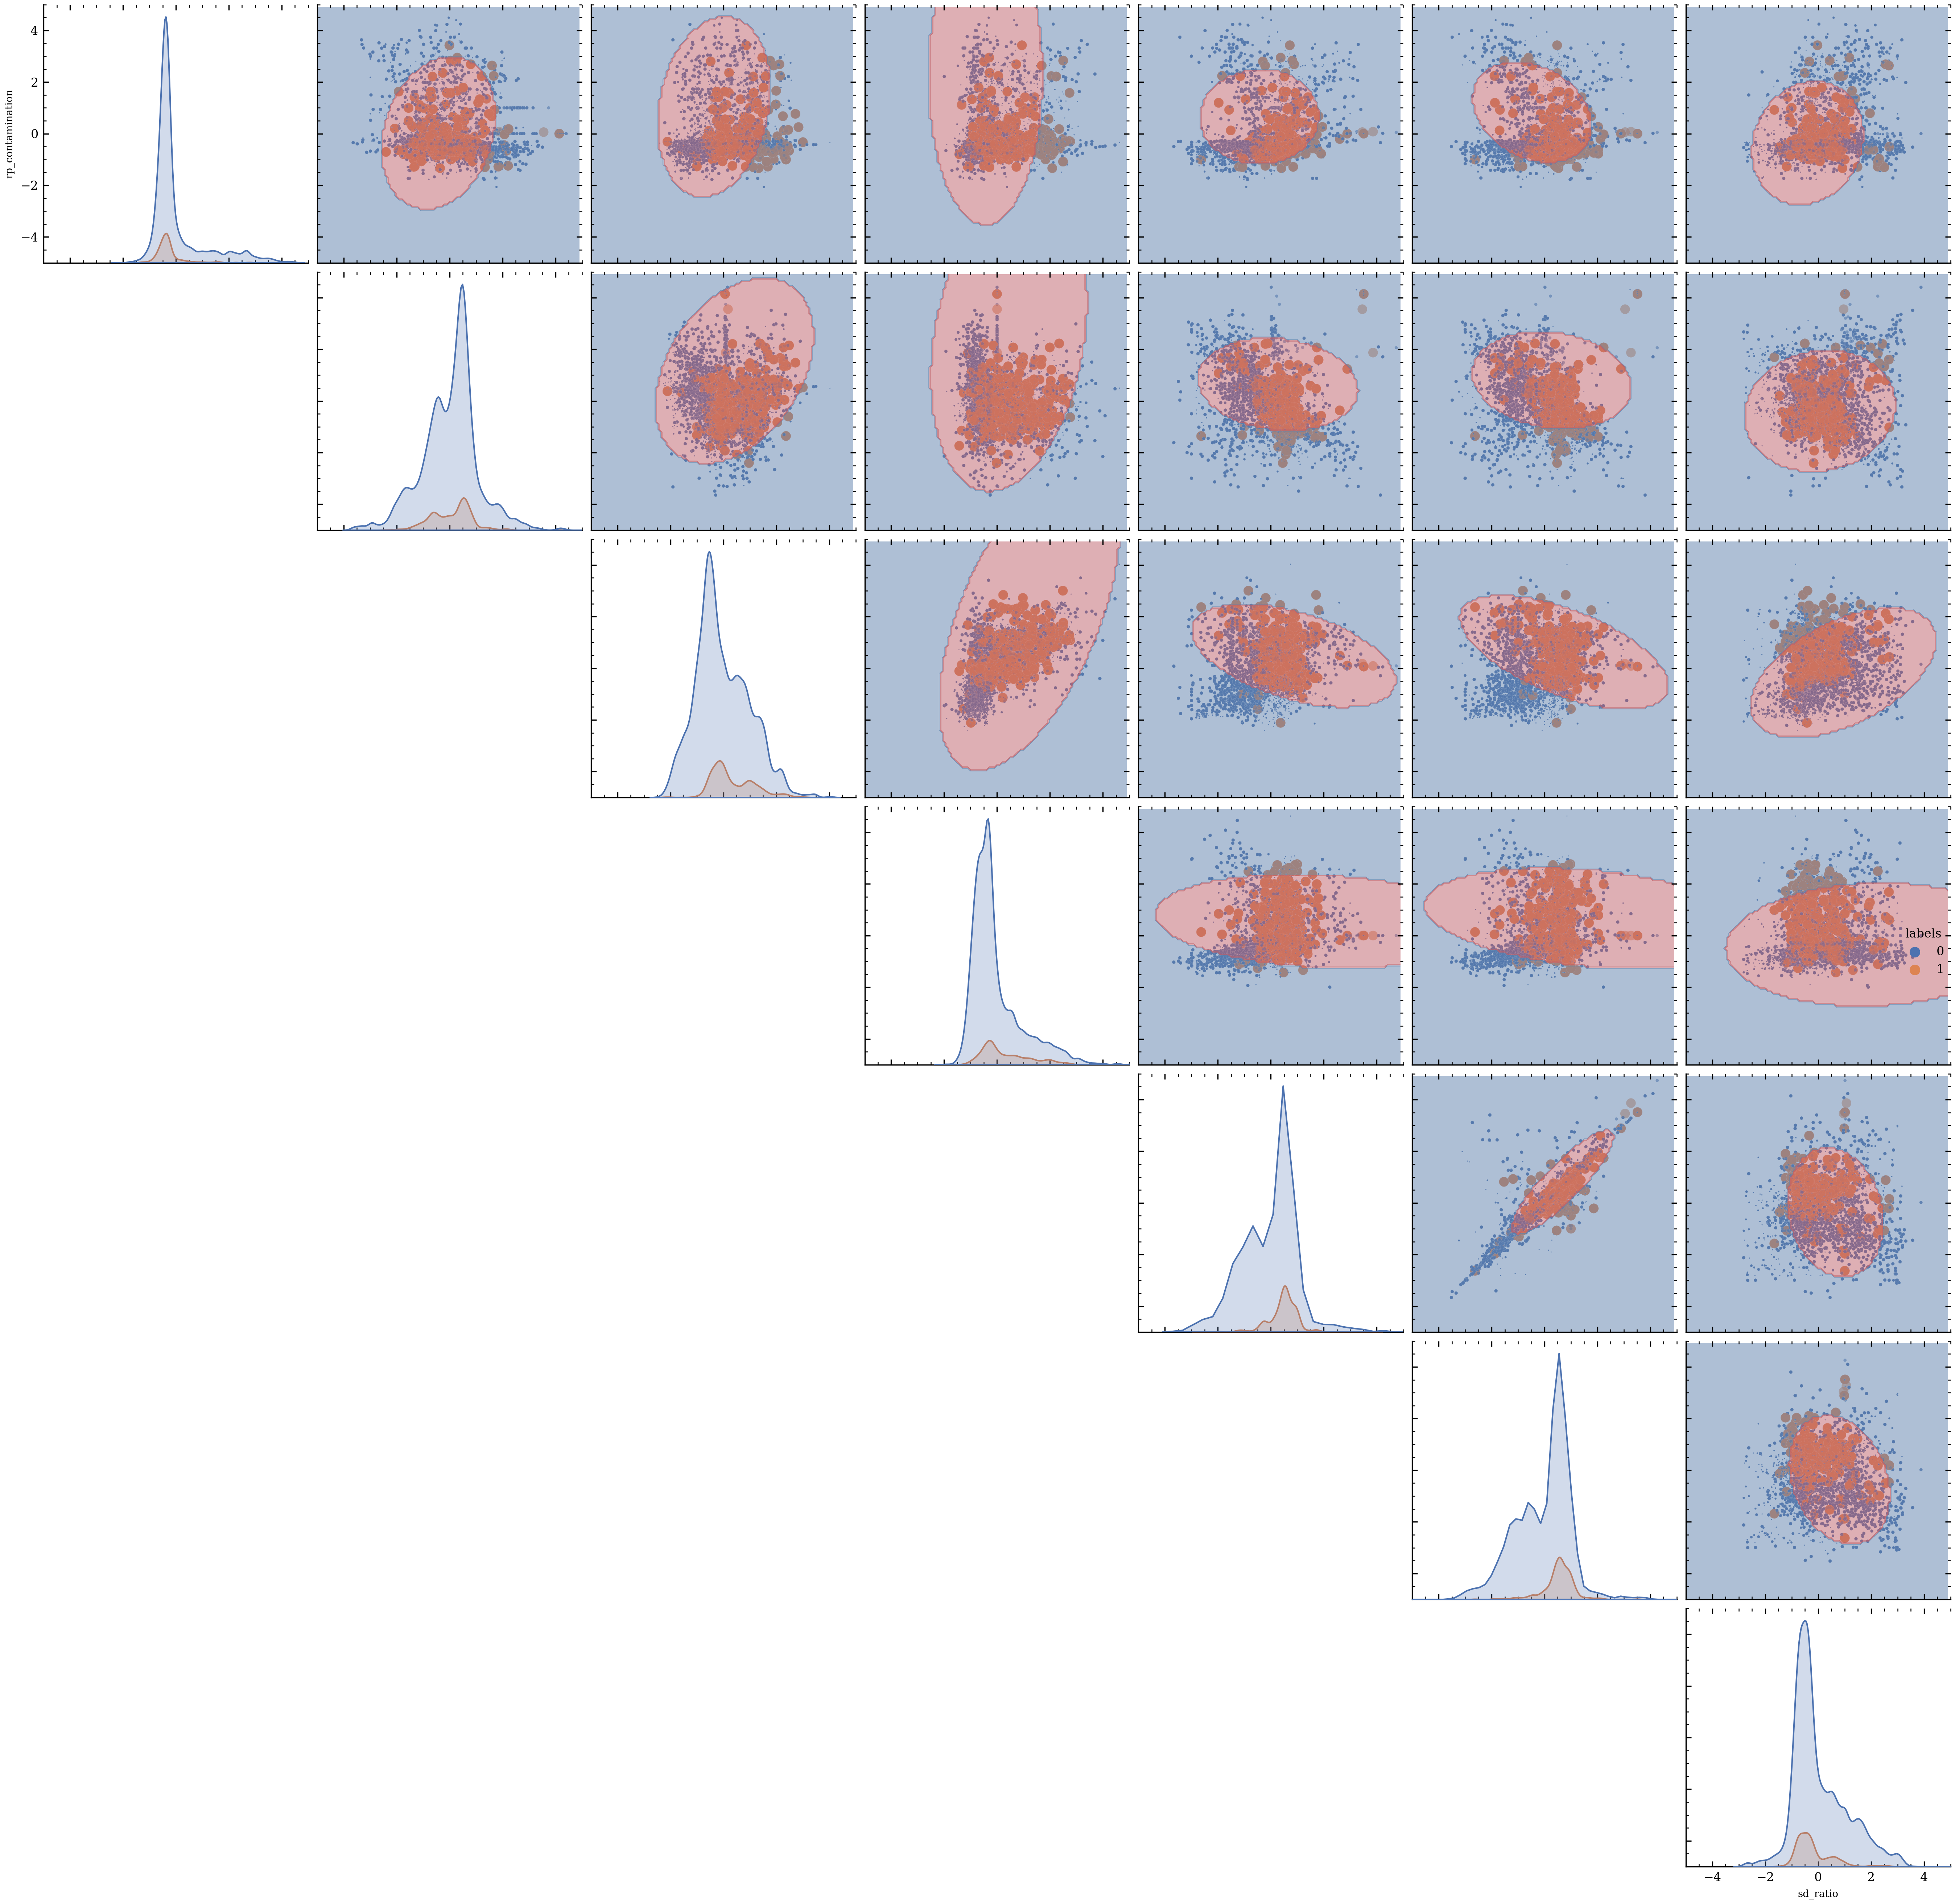
\includegraphics[height=0.6\linewidth]{./figure/qda_pair.png}
    \end{figure}
\end{frame}
\begin{frame}{Quadratic Discriminant Analysis}
    \begin{itemize}
        \item for some diensions the clustering is not perfect.
        \item leads quite to the same results as for the Bayesian approach
        \item one can show that the boundaries are a little less strict
        \item The final score is 0.88.
    \end{itemize}
\end{frame}
\subsubsection{Comparison of the different methods}
\begin{frame}{Comparison of the different methods}
    \begin{itemize}
        \item The different methods lead quite to the same score
        \item However boundaries are a little more strict for the QDA
        \item avoid False negative is more important than avoiding False positive, because we have many points
        \item quadratic discriminant analysis is the best method for tackling the classification problem
    \end{itemize}
\end{frame}
\section{Conclusion}
\begin{frame}{Conclusion}
    \begin{itemize}
        \item The Lussac algorithm is a complex problem, and there is no unique solution.
        \item The goal of the Lussac project is to develop a new spikesorting algorithm that will be able to deal with multiple spikesorting algorithms.
        \item ptimize the Lussac choice between the different spikesorting algorithms.
        \item Two clustering steps are necessary : Clustering of good relations to isolate the neurons clusters and clustering of the neurons to isolate the best neurons of each cluster.
        \item We find the best method in our scope of study
    \end{itemize}
\end{frame}
\end{document}